\documentclass[11pt, oneside, appendixprefix=Appendix]{article}
\usepackage[margin=1in]{geometry}
\geometry{letterpaper}
\usepackage[parfill]{parskip}
\usepackage{graphicx}
\usepackage{amssymb}
\usepackage{amsmath}
\usepackage{amsthm}
\usepackage{scrextend}
\usepackage{tikz}
\usepackage{float}
\usepackage{titlesec}
\usepackage{apacite}
\usepackage{url}
\usepackage{setspace}
\usepackage{titling}
\usepackage{caption}
\usepackage{subcaption}
\usepackage{mathptmx}
\usepackage{mathtools}
\usepackage{pgfplots}
\usepackage[titletoc]{appendix}
\usepackage{array}
\usepackage{chngcntr}
\usepackage{booktabs}

\DeclareMathOperator*{\argmax}{arg\,max}
\DeclareMathOperator*{\argmin}{arg\,min}

\captionsetup[table]{position=bottom}
\counterwithin{table}{section}

\usetikzlibrary{decorations.pathreplacing}

\newcommand{\sectionbreak}{\clearpage}

\doublespacing

\renewcommand\maketitlehooka{\null\mbox{}\vfill}
\renewcommand\maketitlehookd{\vfill\null}

%running fraction with slash - requires math mode.
\newcommand*\rfrac[2]{{}^{#1}\!/_{#2}}

\theoremstyle{definition}
\newtheorem{example_heading}{Example}[section]
\newtheorem{definition_heading}{Definition}
\newtheorem{property_heading}{Property}

\newenvironment{example} % Numbed examples with narrower width
{\begin{quote} \begin{example_heading}}
{\end{example_heading} \end{quote}}

\newenvironment{definition}
{\begin{quote} \begin{definition_heading}}
{\end{definition_heading} \end{quote}}

\newenvironment{property}
{\begin{quote} \begin{property_heading}}
{\end{property_heading} \end{quote}}

\newenvironment{equation_nogap} % Equation with little vertical gaps (https://tex.stackexchange.com/questions/180630/spacing-problem-between-equation-and-surrounding-text)
{\begin{smallskip} \begin{centering} \begin{spacing}{1.0} $} % Not sure why \begin{par} would be necessary, so I removed it.
{$ \end{spacing} \end{centering} \end{smallskip}}

\newenvironment{absnopagebreak} % Absolutely no page break
  {\par\nobreak\vfil\penalty0\vfilneg\vtop\bgroup}
  {\par\xdef\tpd{\the\prevdepth}\egroup\prevdepth=\tpd}

\numberwithin{figure}{section}

\def\bezier(#1,#2, #3, #4, #5){#2*((1-#1)^3) + 3*#3*((1-#1)^2)*#1 + 3*#4*(1-#1)*(#1^2) + #5*(#1^3)}%


\title{How can the B\'ezier curve be used to approximate a cycloid?}
\author{Daekun Kim}
%\date{}							% Activate to display a given date or no date

\begin{document}
\begin{titlingpage}
\maketitle
Word count: 5161
\end{titlingpage}
\tableofcontents
\newpage

%==========================================================================================
%==========================================================================================
%=================================== INTRODUCTION =========================================
%==========================================================================================
%==========================================================================================
\section{Introduction}
	In the modern era, the computers are one of the most influential tools in humanity's lives. In fact, generations born after the 2000s, including myself, hardly lived an era with absence of heavy influence of computers. Many of its powerful abilities, such as being able to render high quality realistic images, is taken for granted by many people. It is capable of displaying millions of polygons and curved shapes in few milliseconds, which is crucial for many industrial applications, 3D video games, and for designers. However, computers, by nature, can only process discrete information, and it seems as if it must be only capable  of rendering straight and rigid shapes; it is not clear how it is possible for them to portray such smooth curved surfaces and shapes in such a swift manner.

This rendering of curves and curved surfaces can be achieved using many methods, but one of the most prominent method is the B\'ezier curve. It is utilized in many of the famous 3D design and animation softwares, such as Adobe Flash \fullcite{FLASH:2012}, GIMP \fullcite{GOELKER:2007}, and Adobe Photoshop \fullcite{FULLER:2007}. Along with being one of the most popular methods to render curves in computer systems, the B\'ezier curves are also relatively intuitive and concise that it can be more easily understood than other more complicated methods, which will be explained throughout this essay.

This essay aims to \textbf{investigate the mathematical development of the B\'ezier curve, a method used to construct curves in computer systems}. I intend to connect the idea of rudimentary linear function to linear interpolation, and its parametric definition. Then, a natural realization of the De Casteljau algorithm, a recursive process used to construct the B\'ezier curve, from a repeated linear interpolation of attempting to draw a curve will be explained. Finally, the definition and the properties of B\'ezier curve itself will be discussed, with thorough examples of its real-world applications. Ultimately, the objective is to examine the development of the B\'ezier curve using the mathematical concepts taught in IB Mathematics HL.

%==========================================================================================
%==========================================================================================
%=================================== LINEAR INTERPOLATION =================================
%==========================================================================================
%==========================================================================================

\section{Linear Interpolation}

Straight lines are one of the easiest shapes one can imagine and draw, because of their simplicity to understand and manipulate. Such holds true even for computers. Graphically, drawing straight lines is the most rudimentary job a computer can perform. However, because it is so easy to render, it forms the fundamentals of how computers can render sophisticated curves and surfaces onto a screen.

Lines can be thought of as the shortest path that connects two points. A \textbf{linear interpolation}, then, is calculating which position on the line one would arrive on if one was to travel certain distance or time. Mathematically, given two points, $(x_A, y_A)$ and $(x_B,y_B)$ with $x_A < x_B$, a linear interpolation is construction of a new set of $y$ from $x$ values within $[x_A, x_B]$. The formula of linear interpolation can be given as a relationship of the slopes of the lines connecting the starting and end point with that of line connecting the interpolated point with the starting point, or

\begin{equation}
\frac{y-y_A}{x-x_A}=\frac{y_B-y_A}{x_B-x_A}
\end{equation}

Eq. (1) is stating that, if a person was to travel over a line, the ratio of the distances at which one travelled vertically over the horizontal distance travelled must be the same no matter the position he or she lies on the line.

\begin{example}

\begin{figure}[H]
	\centering
	\begin{tikzpicture}[scale=1]
		\draw [->] (0,0) -- (0,3) node[align=left, right] {$y$};
		\draw [->] (0,0) -- (4,0) node[align=left, above] {$x$};
		\draw (0,0) node[anchor=north east,fill=white] {0};
		\foreach \x/\xtext in {1, 2, 3} 
			\draw (\x,1pt) -- (\x,-1pt) node[anchor=north,fill=white] {$\xtext$};
		\foreach \y/\ytext in {1, 2} 
			\draw (1pt,\y) -- (-1pt,\y) node[anchor=east,fill=white] {$\ytext$};
		
		\path	(1,1) node(p0) {} 
			(3,2) node(p1) {};
		\draw (p0) -- (p1);
		\filldraw (p0) circle (1pt) node[align=center, below] {$(1,1)$};
		\filldraw (p1) circle (1pt) node[align=center, above] {$(3,2)$};
	\end{tikzpicture}
	\caption{Linear interpolation between two points}
\end{figure}

Fig. 2.1 shows an example of linear interpolation between $(1,1)$ and $(3,2)$.

The equation of linear interpolation in Fig. 2.1 can be defined as following:

\begin{equation}
\frac{y-1}{x-1}=\frac{2-1}{3-1},1 \leq x \leq 2
\end{equation}

The line shown in Fig 2.1 is called the \textbf{interpolant}, which can be thought of, literally, as a shortest path between two points. Solving Eq. (2) for $x$ gives us the following:

\begin{equation}
\begin{split}
y	& = \frac{1}{2}(x-1)+1, \\ 
	& = \frac{1}{2}x+\frac{1}{2}
\end{split}
\end{equation}

In fact, this is now in slope-intercept form of an equation of a linear function, $y=mx+b$! This signifies that linear interpolation is nothing more than a linear function with a restricted domain between two points.

\end{example}


\section{Parametric Equations}
The previous section showed that linear interpolation is essentially plotting a point on a line using a linear function. However, such is not possible with our original definition of linear interpolation when the line cannot be defined using a function. For instance, consider a straight vertical line as shown in Fig 3.1.

\begin{figure}[h]
	\centering
	\begin{tikzpicture}[scale=1]
		\draw [->] (0,0) -- (0,4) node[align=left, right] {$y$};
		\draw [->] (0,0) -- (4,0) node[align=left, above] {$x$};
		\draw (0,0) node[anchor=north east,fill=white] {0};
		\foreach \x/\xtext in {1, 2, 3} 
			\draw (\x,1pt) -- (\x,-1pt) node[anchor=north,fill=white] {$\xtext$};
		\foreach \y/\ytext in {1, 2, 3} 
			\draw (1pt,\y) -- (-1pt,\y) node[anchor=east,fill=white] {$\ytext$};
		
		\path	(2,1) node(p0) {} 
			(2,3) node(p1) {};
		\draw (p0) -- (p1);
		\filldraw (p0) circle (1pt) node[align=center, below] {$(1,1)$};
		\filldraw (p1) circle (1pt) node[align=center, above] {$(3,2)$};
	\end{tikzpicture}
	\caption{A vertical linear interpolation}
\end{figure}

In order for a line to be defined by a function, it must pass the Vertical Line Test, which states that there can only be one and only one $y$ value for each $x$ value. The line shown in Fig 3.1 obviously does not pass this condition, since there are infinitely many $y$ values for $x=2$.

However, by redefining linear interpolation with a set of parametric equations, one can easily overcome this apparent problem. Instead of defining an interpolation with respect to $x$, we can do so with another variable $t$ within $[0,1]$, and define different equations for the values of $y$ and $x$ with no explicitly direct relationship between them. This new variable $t$ can be thought of as the time, or the ratio of how much of the path one have travelled from the initial point to the total distance.

\begin{example}

\begin{figure}[h]
	\centering
	\begin{tikzpicture}[scale=1.5]
		\draw [->] (0,0) -- (0,3) node[align=left, right] {$y$};
		\draw [->] (0,0) -- (4,0) node[align=left, above] {$x$};
		\draw (0,0) node[anchor=north east,fill=white] {0};
		\foreach \x/\xtext in {1, 2, 3} 
			\draw (\x,1pt) -- (\x,-1pt) node[anchor=north,fill=white] {$\xtext$};
		\foreach \y/\ytext in {1, 2} 
			\draw (1pt,\y) -- (-1pt,\y) node[anchor=east,fill=white] {$\ytext$};
		
		\path	(1,1) node(p0) {} 
			(3,2) node(p1) {};
		\filldraw (p0) circle (1pt) node[align=center, below] {$P_A(1,1)$};
		\filldraw (p1) circle (1pt) node[align=center, above] {$P_B(3,2)$};
		\draw (p0) -- (p1);
		\draw (1,1) -- (3,1);
		\draw (1,1) -- (1,2);
		\draw[dashed] (2,1) -- (2,1.5);
		\draw[dashed] (1,1.5) -- (2,1.5);
		\filldraw (2,1.5) circle (1pt) node[align=center, below right] {$P'(2,\frac{3}{2})$};
%		\draw (2,1+0.05) -- (2,1-0.05) node[anchor=north,fill=white] {t=0.5};
		\draw (1.46,1+0.05) -- (1.5,1-0.05);
		\draw (1.5,1+0.05) -- (1.54,1-0.05);
		\draw (2.46,1+0.05) -- (2.5,1-0.05);
		\draw (2.5,1+0.05) -- (2.54,1-0.05);
		\draw (1+0.05,1.23) -- (1-0.05,1.27);
		\draw (1+0.05,1.73) -- (1-0.05,1.77);
	\end{tikzpicture}
	\caption{Parametric linear interpolation for $t=0.5$}
\end{figure}

Fig. 3.2 shows a linear interpolation at $t=0.5$. At $t=0.5$, the resulting point at halfway between $P_A$ and $P_B$ in both directions of the $x$- and $y$-axes. This can be thought of as a driver having travelled 50\% of the path.
\end{example}

\begin{example}

\begin{figure}[H]
	\centering
	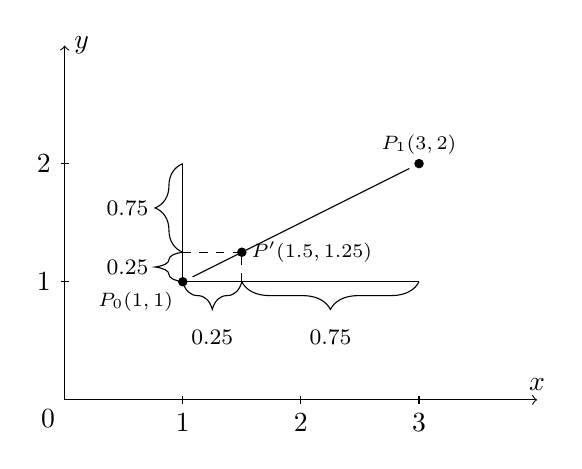
\begin{tikzpicture}[scale=1.5]
		\draw [->] (0,0) -- (0,3) node[align=left, right] {$y$};
		\draw [->] (0,0) -- (4,0) node[align=left, above] {$x$};
		\draw (0,0) node[anchor=north east,fill=white] {0};
		\foreach \x/\xtext in {1, 2, 3} 
			\draw (\x,1pt) -- (\x,-1pt) node[anchor=north,fill=white] {$\xtext$};
		\foreach \y/\ytext in {1, 2} 
			\draw (1pt,\y) -- (-1pt,\y) node[anchor=east,fill=white] {$\ytext$};
		
		\path	(1,1) node(p0) {} 
			(3,2) node(p1) {};
		\filldraw (p0) circle (1pt) node[align=center, below left] {\scriptsize $P_0(1,1)$};
		\filldraw (p1) circle (1pt) node[align=center, above] {\scriptsize $P_1(3,2)$};
		\draw (p0) -- (p1);
		\draw (1,1) -- (3,1);
		\draw (1,1) -- (1,2);
		\draw[dashed] (1.5,1) -- (1.5,1.25);
		\draw[dashed] (1,1.25) -- (1.5,1.25);
		\filldraw (1.5,1.25) circle (1pt) node[align=center, right] {\scriptsize $P'(1.5,1.25)$};
		\draw [decorate,decoration={brace,amplitude=10pt,mirror},xshift=0pt,yshift=0pt] (1,1) -- (1.5,1) node [black,midway,yshift=-20pt] {\footnotesize $0.25$};
		\draw [decorate,decoration={brace,amplitude=10pt,mirror},xshift=0pt,yshift=0pt] (1.5,1) -- (3,1) node [black,midway,yshift=-20pt] {\footnotesize $0.75$};
		
		\draw [decorate,decoration={brace,amplitude=10pt},xshift=0pt,yshift=0pt] (1,1) -- (1,1.25) node [black,midway,xshift=-20pt] {\footnotesize $0.25$};
		\draw [decorate,decoration={brace,amplitude=10pt},xshift=0pt,yshift=0pt] (1,1.25) -- (1,2) node [black,midway,xshift=-20pt] {\footnotesize $0.75$};
	\end{tikzpicture}
	\caption{Parametric linear interpolation for $t=0.25$}
\end{figure}

In the same way, as shown in Fig. 3.3, at $t=0.25$, the resulting points are one-quarter of the way between the initial and the terminal points in both axes, which is like travelling 25\% of the path since the starting point.
\end{example}

As shown in the two examples above, the $t$ value is analogous to the ratio in which the person has travelled from the initial point that a GPS device would let one know.

As such, a linear interpolation between $(x_A, y_B)$ and $(x_A,y_B)$ can be parametrically defined as following:
\begin{gather}
x(t)=x_A + (x_B - x_A)t \\
y(t)=y_A + (y_B - y_A)t
\end{gather}

At $t=0$, the interpolated point is at $(x_A, y_A)$, the initial point, and at $t=0$, it is at $(x_1,y_1)$, the terminal point. This can be considered as being at the initial point when one has travelled 0\% of the path, and as being at the terminal point when one has travelled 100\% of the path.

Parametric equations (4) and (5), however, look to be very similar. In fact, they can be combined to form a 2-dimensional (2D) vector equation. Let $P_0$ and $P_1$ be position vectors, where $P_0=(x_0,y_0)$ and $P_1=(x_1,y_1)$. Then,

\begin{equation}
P(t)=P_0 + (P_1 - P_0)t,
\end{equation}

where $P(t)$ is a function that linearly interpolates a point between $P_0$ and $P_1$ for $t \in [0,1]$. Analogously, this is a vector addition between the initial location and the path a driver has travelled so far at time $t$. Eq. (6) can be rearranged as following:

\begin{equation}
P(t)={P_0}(1-t) + {P_1}t,
\end{equation}

Eq. (7) further emphasizes the analogous nature of $t$ being the ``ratio'' \fullcite{PRAUTZ:2013} of the resulting point $P$ with respect to the initial and final points. More specifically, the ratio $t:(1-t)$ equals to the ratio of the distance from the current point $P$ with the initial point $P_0$ and the final point $P_1$, respectively, as shown in Fig. 3.4.

\begin{figure}[H]
	\centering
	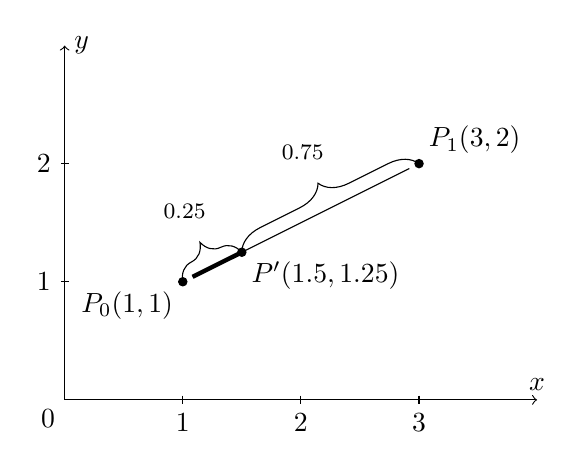
\begin{tikzpicture}[scale=1.5]
		\draw [->] (0,0) -- (0,3) node[align=left, right] {$y$};
		\draw [->] (0,0) -- (4,0) node[align=left, above] {$x$};
		\draw (0,0) node[anchor=north east,fill=white] {0};
		\foreach \x/\xtext in {1, 2, 3} 
			\draw (\x,1pt) -- (\x,-1pt) node[anchor=north,fill=white] {$\xtext$};
		\foreach \y/\ytext in {1, 2} 
			\draw (1pt,\y) -- (-1pt,\y) node[anchor=east,fill=white] {$\ytext$};
		
		\path	(1,1) node(p0) {} 
			(3,2) node(p1) {};
		\filldraw (p0) circle (1pt) node[align=center, below left] {$P_0(1,1)$};
		\filldraw (p1) circle (1pt) node[align=center, above right] {$P_1(3,2)$};
		\draw (p0) -- (p1);
		\draw[ultra thick] (p0) -- (1.5,1.25);
		\filldraw (1.5,1.25) circle (1pt) node[align=center, below right] {$P'(1.5,1.25)$};
		
		\draw [decorate,decoration={brace,amplitude=10pt},xshift=0pt,yshift=0pt] (1,1) -- (1.5,1.25) node [black,midway,yshift=20pt,xshift=-10pt] {\footnotesize $0.25$};
		\draw [decorate,decoration={brace,amplitude=10pt},xshift=0pt,yshift=0pt] (1.5,1.25) -- (3,2) node [black,midway,yshift=20pt,xshift=-10pt] {\footnotesize $0.75$};
	\end{tikzpicture}
	\caption{Ratio of $(1-t)$ and $t$ for $t=0.25$}
\end{figure}

To construct the interpolant, $t$ values with an infinitesimal interval between each other would be used. In computer systems, this would translate to having $t$ values with an interval small enough that will allow the line to appear smooth and continuous, and large enough to not harm the performance of the computer.

\section{Recursive Linear Interpolation}

Thus far, the main focus of our investigation was on the methods used to produce straight lines. However, surprisingly, linear interpolation can be repeated to produce a smooth curve. The following example will show how such can be achieved with 3 points.

\begin{example} Let $P_0 = (1,1)$, $P_1 = (2,2)$, and $P_2 = (3,1)$. By applying linear interpolation, we know that we can produce straight lines between these three points using the vector equation $P(t) = P_A(1-t) + P_{B}t$. This is shown in Fig. 4.1.

\begin{figure}[H]
	\centering
	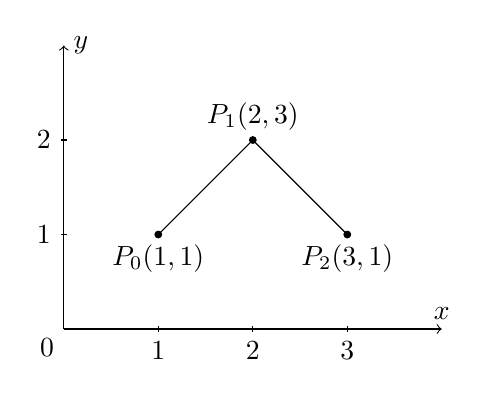
\begin{tikzpicture}[scale=1.2]
		\draw [->] (0,0) -- (0,3) node[align=left, right] {$y$};
		\draw [->] (0,0) -- (4,0) node[align=left, above] {$x$};
		\draw (0,0) node[anchor=north east,fill=white] {0};
		\foreach \x/\xtext in {1, 2, 3} 
			\draw (\x,1pt) -- (\x,-1pt) node[anchor=north,fill=white] {$\xtext$};
		\foreach \y/\ytext in {1, 2} 
			\draw (1pt,\y) -- (-1pt,\y) node[anchor=east,fill=white] {$\ytext$};
		
		\filldraw (1,1) circle (1pt) node[align=center, below] {$P_0(1,1)$};
		\filldraw (2,2) circle (1pt) node[align=center, above] {$P_1(2,3)$};
		\filldraw (3,1) circle (1pt) node[align=center, below] {$P_2(3,1)$};
		
		\draw (1,1) -- (2,2) -- (3,1);
	\end{tikzpicture}
	\caption{Linear interpolants between $P_0$ and $P_1$, and $P_1$ and $P_2$}
\end{figure}

Let $P_{0 \dotsc 1}$ be a linearly interpolated point between $P_0$ and $P_1$ at $t=0.5$. Similarly, let $P_{1 \dotsc 2}$ be the linearly interpolated point between $P_1$ and $P_2$ at $t=0.5$. These newly interpolated points can be used as the starting and terminal points of new linear interpolation, as shown in Fig. 4.2.

\begin{figure}[H]
	\centering
	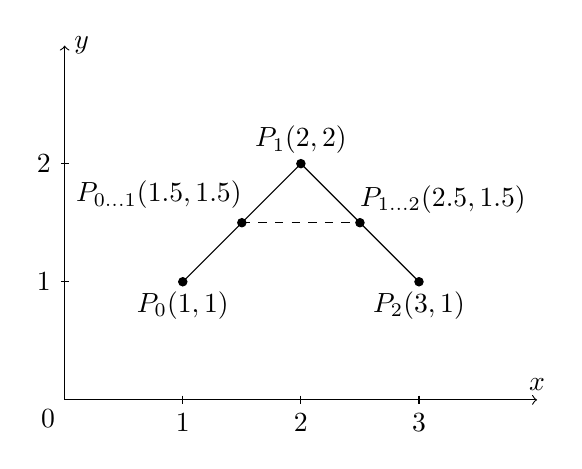
\begin{tikzpicture}[scale=1.5]
%	\begin{scriptsize}
		\draw [->] (0,0) -- (0,3) node[align=left, right] {$y$};
		\draw [->] (0,0) -- (4,0) node[align=left, above] {$x$};
		\draw (0,0) node[anchor=north east,fill=white] {0};
		\foreach \x/\xtext in {1, 2, 3} 
			\draw (\x,1pt) -- (\x,-1pt) node[anchor=north,fill=white] {$\xtext$};
		\foreach \y/\ytext in {1, 2} 
			\draw (1pt,\y) -- (-1pt,\y) node[anchor=east,fill=white] {$\ytext$};
		
		\filldraw (1,1) circle (1pt) node[align=center, below] {$P_0(1,1)$};
		\filldraw (2,2) circle (1pt) node[align=center, above] {$P_1(2,2)$};
		\filldraw (3,1) circle (1pt) node[align=center, below] {$P_2(3,1)$};
		
		\draw (1,1) -- (2,2) -- (3,1);
		
		\filldraw (1.5,1.5) circle (1pt) node[align=center, xshift=-30pt, yshift=10pt] {$P_{0 \dotsc 1}(1.5,1.5)$};
		\filldraw (2.5,1.5) circle (1pt) node[align=center, xshift=30pt, above] {$P_{1 \dotsc 2}(2.5,1.5)$};
		\draw[dashed] (1.5,1.5) -- (2.5,1.5);
%	\end{scriptsize}
	\end{tikzpicture}
	\caption{Linear interpolant of $P_{0 \dotsc 1}$ and $P_{1 \dotsc 2}$}
\end{figure}

Finally, let $P_{0 \dotsc 2}$ be the linearly interpolated point between $P_{0 \dotsc 1}$ and $P_{1 \dotsc 2}$. $P_{0 \dotsc 2}$, then, is a resulting point of the quadratic interpolation from points $P_0$, $P_1$, and $P_2$ at $t=0.5$, as shown in Fig. 4.3.

\begin{figure}[H]
	\centering
	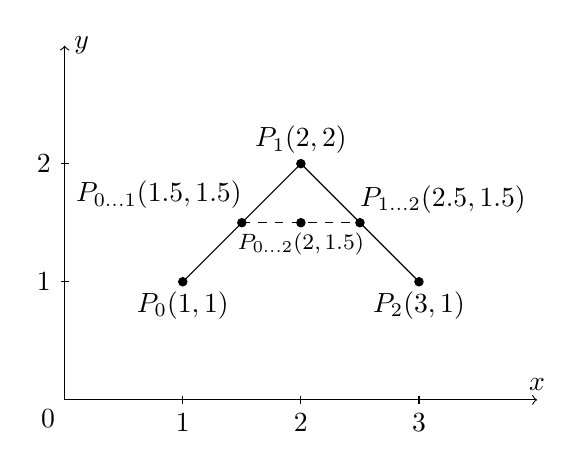
\begin{tikzpicture}[scale=1.5]
%	\begin{scriptsize}
		\draw [->] (0,0) -- (0,3) node[align=left, right] {$y$};
		\draw [->] (0,0) -- (4,0) node[align=left, above] {$x$};
		\draw (0,0) node[anchor=north east,fill=white] {0};
		\foreach \x/\xtext in {1, 2, 3} 
			\draw (\x,1pt) -- (\x,-1pt) node[anchor=north,fill=white] {$\xtext$};
		\foreach \y/\ytext in {1, 2} 
			\draw (1pt,\y) -- (-1pt,\y) node[anchor=east,fill=white] {$\ytext$};
		
		\filldraw (1,1) circle (1pt) node[align=center, below] {$P_0(1,1)$};
		\filldraw (2,2) circle (1pt) node[align=center, above] {$P_1(2,2)$};
		\filldraw (3,1) circle (1pt) node[align=center, below] {$P_2(3,1)$};
		
		\draw (1,1) -- (2,2) -- (3,1);
		
		\filldraw (1.5,1.5) circle (1pt) node[align=center, xshift=-30pt, yshift=10pt] {$P_{0 \dotsc 1}(1.5,1.5)$};
		\filldraw (2.5,1.5) circle (1pt) node[align=center, xshift=30pt, above] {$P_{1 \dotsc 2}(2.5,1.5)$};
		\draw[dashed] (1.5,1.5) -- (2.5,1.5);
		
		\filldraw (2,1.5) circle (1pt) node[align=center, xshift=0pt, below] {\footnotesize $P_{0 \dotsc 2}(2,1.5)$};
%	\end{scriptsize}
	\end{tikzpicture}
	\caption{Quadratic interpolation at $t=0.5$}
\end{figure}

This technique of repeated linear interpolation can be performed at $t=0.25$ and $t=0.75$, as shown in Fig. 4.4 and 4.5.

\begin{figure}[H]
	\centering
	\begin{minipage}{.5\textwidth}
	\centering
	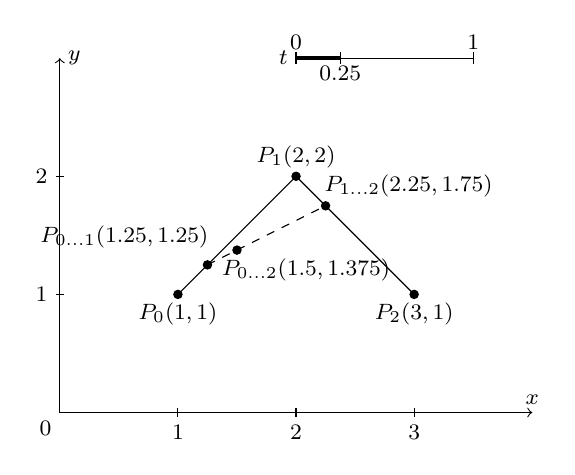
\begin{tikzpicture}[scale=1.5]
	\begin{footnotesize}
		\draw (2,3) -- (3.5, 3) node[pos=0, left]{$t$} node[pos=0, above]{0} node[pos=0.25, below]{0.25} node[pos=1, above]{1};
		\draw[ultra thick] (2,3) -- (2.375, 3);
		\draw (2,3-0.05) -- (2,3+0.05);
		\draw (2.375,3-0.05) -- (2.375,3+0.05);
		\draw (3.5,3-0.05) -- (3.5,3+0.05);
		
		\draw [->] (0,0) -- (0,3) node[align=left, right] {$y$};
		\draw [->] (0,0) -- (4,0) node[align=left, above] {$x$};
		\draw (0,0) node[anchor=north east,fill=white] {0};
		\foreach \x/\xtext in {1, 2, 3} 
			\draw (\x,1pt) -- (\x,-1pt) node[anchor=north,fill=white] {$\xtext$};
		\foreach \y/\ytext in {1, 2} 
			\draw (1pt,\y) -- (-1pt,\y) node[anchor=east,fill=white] {$\ytext$};
		
		\filldraw (1,1) circle (1pt) node[align=center, below] {$P_0(1,1)$};
		\filldraw (2,2) circle (1pt) node[align=center, above] {$P_1(2,2)$};
		\filldraw (3,1) circle (1pt) node[align=center, below] {$P_2(3,1)$};
		
		\draw (1,1) -- (2,2) -- (3,1);
		
		\filldraw (1.25,1.25) circle (1pt) node[align=center, xshift=-30pt, yshift=10pt] {$P_{0 \dotsc 1}(1.25,1.25)$};
		\filldraw (2.25,1.75) circle (1pt) node[align=center, xshift=30pt, above] {$P_{1 \dotsc 2}(2.25,1.75)$};
		\draw[dashed] (1.25,1.25) -- (2.25,1.75);
		
		\filldraw (1.5,1.375) circle (1pt) node[align=center, xshift=25pt, below] { $P_{0 \dotsc 2}(1.5,1.375)$};
	\end{footnotesize}
	\end{tikzpicture}
	\captionof{figure}{\small Quadratic interpolation at $t=0.25$}
	\end{minipage}%
	\begin{minipage}{.5\textwidth}
    		\centering
    		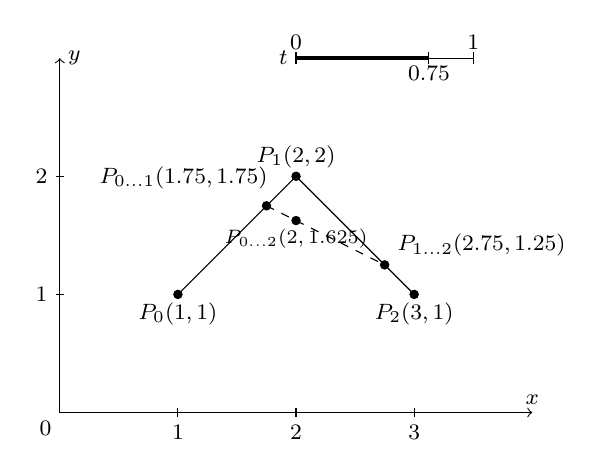
\begin{tikzpicture}[scale=1.5]
    		\begin{footnotesize}
    			\draw (2,3) -- (3.5, 3) node[pos=0, left]{$t$} node[pos=0, above]{0} node[pos=0.75, below]{0.75} node[pos=1, above]{1};
	    		\draw[ultra thick] (2,3) -- (3.125, 3);
	    		\draw (2,3-0.05) -- (2,3+0.05);
	    		\draw (3.125,3-0.05) -- (3.125,3+0.05);
	    		\draw (3.5,3-0.05) -- (3.5,3+0.05);
    		
	    		\draw [->] (0,0) -- (0,3) node[align=left, right] {$y$};
	    		\draw [->] (0,0) -- (4,0) node[align=left, above] {$x$};
	    		\draw (0,0) node[anchor=north east,fill=white] {0};
	    		\foreach \x/\xtext in {1, 2, 3} 
    			\draw (\x,1pt) -- (\x,-1pt) node[anchor=north,fill=white] {$\xtext$};
	    		\foreach \y/\ytext in {1, 2} 
	    			\draw (1pt,\y) -- (-1pt,\y) node[anchor=east,fill=white] {$\ytext$};
	    		
	    		\filldraw (1,1) circle (1pt) node[align=center, below] {$P_0(1,1)$};
	    		\filldraw (2,2) circle (1pt) node[align=center, above] {$P_1(2,2)$};
	    		\filldraw (3,1) circle (1pt) node[align=center, below] {$P_2(3,1)$};
	    		
	    		\draw (1,1) -- (2,2) -- (3,1);
	    		
	    		\filldraw (1.75,1.75) circle (1pt) node[align=center, xshift=-30pt, yshift=10pt] {$P_{0 \dotsc 1}(1.75,1.75)$};
	    		\filldraw (2.75,1.25) circle (1pt) node[align=center, xshift=35pt, above] {$P_{1 \dotsc 2}(2.75,1.25)$};
	    		\draw[dashed] (1.75,1.75) -- (2.75,1.25);
	    		
	    		\filldraw (2,1.625) circle (1pt) node[align=center, below] {\scriptsize $P_{0 \dotsc 2}(2,1.625)$};
	    	\end{footnotesize}
	    	\end{tikzpicture}
	    	\captionof{figure}{\small Quadratic interpolation at $t=0.75$}
	\end{minipage}
\end{figure}

\end{example}

At $t=0$ and $t=1$, the quadratic interpolation always yields points identical to the first and last of the original point, respectively.

\begin{example} The points $P_0$, $P_1$ and $P_2$ are defined as that of example 4.1. At $t=0$, the two linearly interpolated points are

\begin{equation_nogap}\begin{aligned}
P_{0 \dotsc 1}(0)	& = P_0(1-0) + P_1(0) \\
			& = P_0.\\
P_{1 \dotsc 2}(0)	& = P_1(1-0) + P_2(0) \\
			& = P_1. \\
			\\
\end{aligned}\end{equation_nogap}

Then, the resulting point from the quadratic interpolation is

\begin{equation_nogap}\begin{aligned}
P_{0 \dotsc 2}(0)	& = P_{0 \dotsc 1}(1-0) + P_{1 \dotsc 2}(0) \\
			& = P_{0 \dotsc 1} \\
			& = P_0, \\
			\\
\end{aligned}\end{equation_nogap}

which is the first of the original points, $P_0$.
\end{example}

\begin{example} Given the same three points as Examples 4.1 and 4.2, at $t=1$, the two linearly interpolated points are

\begin{equation_nogap}\begin{aligned}
P_{0 \dotsc 1}(1)	& = P_0(1-1) + P_1(1) \\
			& = P_1.\\
P_{1 \dotsc 2}(1)	& = P_1(1-1) + P_2(1) \\
			& = P_2. \\
			\\
\end{aligned}\end{equation_nogap}

Then, the resulting point from the quadratic interpolation is

\begin{equation_nogap}\begin{aligned}
P_{0 \dotsc 2}(1)	& = P_{0 \dotsc 1}(1-1) + P_{1 \dotsc 2}(1) \\
			& = P_{1 \dotsc 2} \\
			& = P_2, \\
\\
\end{aligned}\end{equation_nogap}

which is the last of the original points, $P_2$.
\end{example}

With infinitesimal interval of $t$ values, the quadratic interpolant can be consturcted, as shown in Fig. 4.6. In computer systems, this would translate to having small enough interval of $t$ value that will allow the curve to look smooth, and also one that is large enough that will not harm the computer's performance with redundant calculations.

\begin{figure}[H]
	\centering
	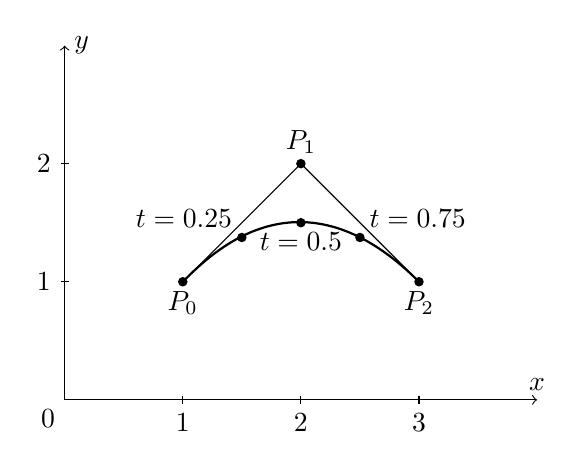
\begin{tikzpicture}[scale=1.5]
		\draw [->] (0,0) -- (0,3) node[align=left, right] {$y$};
		\draw [->] (0,0) -- (4,0) node[align=left, above] {$x$};
		\draw (0,0) node[anchor=north east,fill=white] {0};
		\foreach \x/\xtext in {1, 2, 3} 
			\draw (\x,1pt) -- (\x,-1pt) node[anchor=north,fill=white] {$\xtext$};
		\foreach \y/\ytext in {1, 2} 
			\draw (1pt,\y) -- (-1pt,\y) node[anchor=east,fill=white] {$\ytext$};
		
		\filldraw (1,1) circle (1pt) node[align=center, below] {$P_0$};
		\filldraw (2,2) circle (1pt) node[align=center, above] {$P_1$};
		\filldraw (3,1) circle (1pt) node[align=center, below] {$P_2$};
		
		\draw (1,1) -- (2,2) -- (3,1);
		
		\filldraw (2,1.5) circle (1pt) node[align=center, below] {$t=0.5$};
		\filldraw (1.5,1.375) circle (1pt) node[align=center, above left] {$t=0.25$};
		\filldraw (2.5,1.375) circle (1pt) node[align=center, above right] {$t=0.75$};
		
		\draw[thick] (1,1) .. controls (1.25,1.25) and (2,2) .. (3,1);
	\end{tikzpicture}
	\caption{Quadratic interpolant}
\end{figure}

This repeated linear interpolation is called the \textbf{De Casteljau construction}, or the \textbf{De Casteljau algorithm} \cite{DECAST:1959}. Because this algorithm repeats itself by producing new interpolation from previously interpolated points, it is described as being "recursive" \cite{PRAUTZ:2013}, meaning that it repeats itself to meet the objective. The curve produced from this construction is later formalized and popularized by Pierre B\'ezier \fullcite{FARIN:2001}, by whom this curve, the \textbf{B\'ezier curve}, was named after.

In the De Casteljau algorithm, the only information needed to construct any curve is the initial points, such as $P_0, P_1$ and $P_2$ shown in Fig. 4.6. As such, they are the ones that controls the appearance of the resulting curve. Hence, these points are referred to as the \textbf{control points} of the B\'ezier curve \cite{PRAUTZ:2013}.

Thus far, we have investigated on construction of quadratic curves with three B\'ezier control points. However, by following the similar process of repeating linear interpolation, curves with higher number of control points can be easily constructed, as shown in the following example.

\begin{example} Let $P_0 = (1, 1), P_1 = (1, 5), P_2 = (5, 5),$ and $P_3 = (5, 1)$. With linear interpolation performed for each consecutive pairs of control points, a set of straight interpolants can be produced as shown in Fig. 4.7.

\begin{figure}[H]
	\centering
	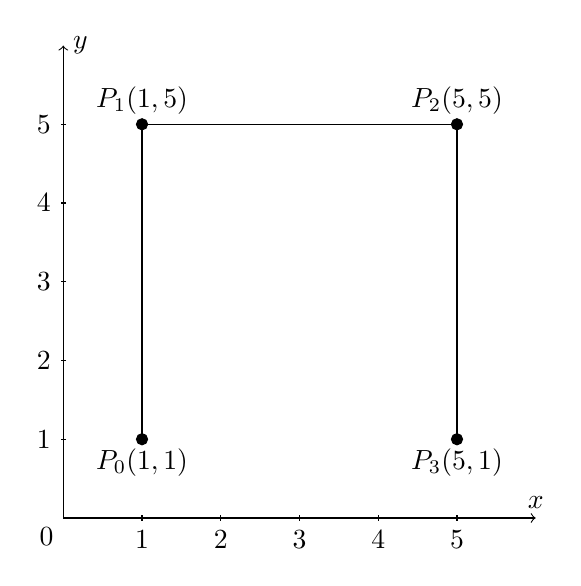
\begin{tikzpicture}[scale=1]
		\coordinate (P_0) at (1, 1);
		\coordinate (P_1) at (1, 5);
		\coordinate (P_2) at (5, 5);
		\coordinate (P_3) at (5, 1);
		
		\draw [->] (0,0) -- (0,6) node[align=left, right] {$y$};
		\draw [->] (0,0) -- (6,0) node[align=left, above] {$x$};
		\draw (0,0) node[anchor=north east,fill=white] {0};
		\foreach \x/\xtext in {1, 2, 3, 4, 5} 
			\draw (\x,1pt) -- (\x,-1pt) node[anchor=north,fill=white] {$\xtext$};
		\foreach \y/\ytext in {1, 2, 3, 4, 5} 
			\draw (1pt,\y) -- (-1pt,\y) node[anchor=east,fill=white] {$\ytext$};
		
		\draw (P_0) -- (P_1) -- (P_2) -- (P_3);
		
		\filldraw (P_0) circle (2pt) node[align=center, below] {$P_0(1,1)$};
		\filldraw (P_1) circle (2pt) node[align=center, above] {$P_1(1,5)$};
		\filldraw (P_2) circle (2pt) node[align=center, above] {$P_2(5,5)$};
		\filldraw (P_3) circle (2pt) node[align=center, below] {$P_3(5,1)$};
	\end{tikzpicture}
	\caption{Linear interpolants between the four B\'ezier control points}
\end{figure}

In order to produce an interpolated point using the control points, the points $P_{0 \dotsc 1}, P_{1 \dotsc 2}$ and $P_{2 \dotsc 3}$ must be interpolated first. These points can be used to perform another set of linear interpolations, as shown in Fig. 4.8.

\begin{figure}[H]
	\centering
	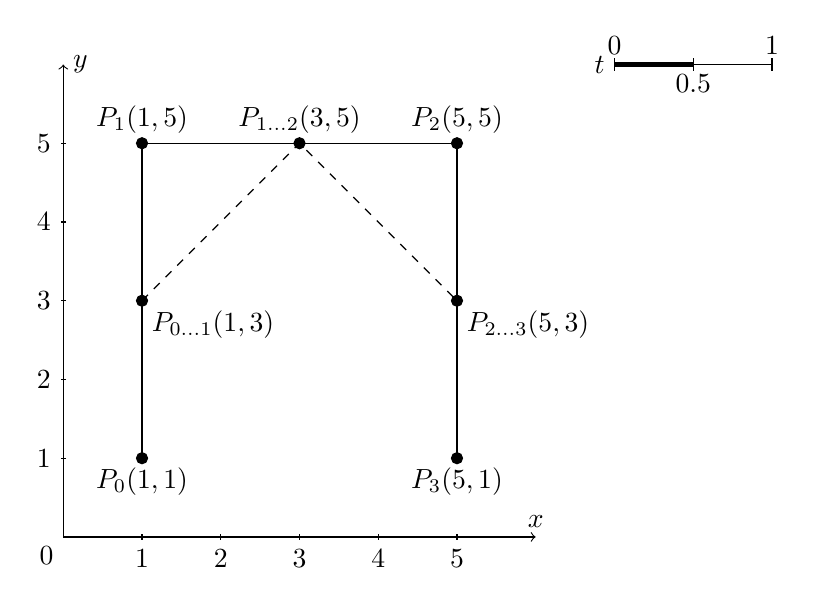
\begin{tikzpicture}[scale=1]
		% Coordinates
		\coordinate (P_0) at (1, 1);
		\coordinate (P_1) at (1, 5);
		\coordinate (P_2) at (5, 5);
		\coordinate (P_3) at (5, 1);
		
		\coordinate (P_0-1) at (1, 3);
		\coordinate (P_1-2) at (3, 5);
		\coordinate (P_2-3) at (5, 3);
		
		% Draw X and Y axes
		\draw [->] (0,0) -- (0,6) node[align=left, right] {$y$};
		\draw [->] (0,0) -- (6,0) node[align=left, above] {$x$};
		\draw (0,0) node[anchor=north east,fill=white] {0};
		\foreach \x/\xtext in {1, 2, 3, 4, 5} 
			\draw (\x,1pt) -- (\x,-1pt) node[anchor=north,fill=white] {$\xtext$};
		\foreach \y/\ytext in {1, 2, 3, 4, 5} 
			\draw (1pt,\y) -- (-1pt,\y) node[anchor=east,fill=white] {$\ytext$};
			
		% Draw t line
		\draw (7,6) -- (9, 6) node[pos=0, left]{$t$} node[pos=0, above]{0} node[pos=0.5, below]{0.5} node[pos=1, above]{1};
	    	\foreach \t/\ttext in {7, 8, 9}
			\draw (\t, 6+0.08) -- (\t, 6-0.08);
		\draw[ultra thick] (7, 6) -- (8, 6);
		
		% First interpolation
		\draw (P_0) -- (P_1) -- (P_2) -- (P_3);
		
		\filldraw (P_0) circle (2pt) node[align=center, below] {$P_0(1,1)$};
		\filldraw (P_1) circle (2pt) node[align=center, above] {$P_1(1,5)$};
		\filldraw (P_2) circle (2pt) node[align=center, above] {$P_2(5,5)$};
		\filldraw (P_3) circle (2pt) node[align=center, below] {$P_3(5,1)$};
		
		% Second Interpolation
		\draw[dashed] (P_0-1) -- (P_1-2) -- (P_2-3);
		
		\filldraw (P_0-1) circle (2pt) node[align=center, below right] {$P_{0 \dotsc 1}(1,3)$};
		\filldraw (P_1-2) circle (2pt) node[align=center, above] {$P_{1 \dotsc 2}(3,5)$};
		\filldraw (P_2-3) circle (2pt) node[align=center, below right] {$P_{2 \dotsc 3}(5,3)$};
	\end{tikzpicture}
	\caption{Second recursion of De Casteljau algorithm}
\end{figure}

Then, the points $P_{0 \dotsc 1}, P_{1 \dotsc 2}$ and $P_{2 \dotsc 3}$ can be used to perform another linear interpolation, as shown in Fig. 4.9.

\begin{figure}[H]
	\centering
	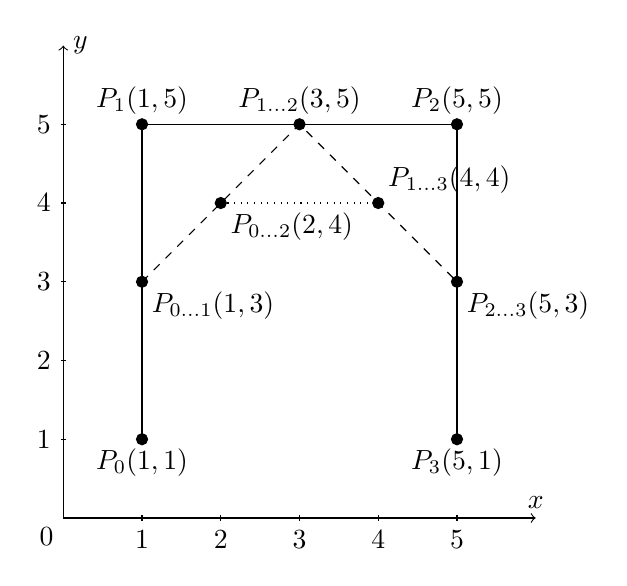
\begin{tikzpicture}[scale=1]
		% Coordinates
		\coordinate (P_0) at (1, 1);
		\coordinate (P_1) at (1, 5);
		\coordinate (P_2) at (5, 5);
		\coordinate (P_3) at (5, 1);
		
		\coordinate (P_0-1) at (1, 3);
		\coordinate (P_1-2) at (3, 5);
		\coordinate (P_2-3) at (5, 3);
		
		\coordinate (P_0-2) at (2, 4);
		\coordinate (P_1-3) at (4, 4);
		
		% Draw X and Y axes
		\draw [->] (0,0) -- (0,6) node[align=left, right] {$y$};
		\draw [->] (0,0) -- (6,0) node[align=left, above] {$x$};
		\draw (0,0) node[anchor=north east,fill=white] {0};
		\foreach \x/\xtext in {1, 2, 3, 4, 5} 
			\draw (\x,1pt) -- (\x,-1pt) node[anchor=north,fill=white] {$\xtext$};
		\foreach \y/\ytext in {1, 2, 3, 4, 5} 
			\draw (1pt,\y) -- (-1pt,\y) node[anchor=east,fill=white] {$\ytext$};
			
		% First interpolation
		\draw (P_0) -- (P_1) -- (P_2) -- (P_3);
		
		\filldraw (P_0) circle (2pt) node[align=center, below] {$P_0(1,1)$};
		\filldraw (P_1) circle (2pt) node[align=center, above] {$P_1(1,5)$};
		\filldraw (P_2) circle (2pt) node[align=center, above] {$P_2(5,5)$};
		\filldraw (P_3) circle (2pt) node[align=center, below] {$P_3(5,1)$};
		
		% Second Interpolation
		\draw[dashed] (P_0-1) -- (P_1-2) -- (P_2-3);
		
		\filldraw (P_0-1) circle (2pt) node[align=center, below right] {$P_{0 \dotsc 1}(1,3)$};
		\filldraw (P_1-2) circle (2pt) node[align=center, above] {$P_{1 \dotsc 2}(3,5)$};
		\filldraw (P_2-3) circle (2pt) node[align=center, below right] {$P_{2 \dotsc 3}(5,3)$};
		
		% Third Interpolation
		\draw[dotted] (P_0-2) -- (P_1-3);
		
		\filldraw (P_0-2) circle (2pt) node[align=center, below right] {$P_{0 \dotsc 2}(2,4)$};
		\filldraw (P_1-3) circle (2pt) node[align=center, above right] {$P_{1 \dotsc 3}(4,4)$};
	\end{tikzpicture}
	\caption{Third recursion of De Casteljau algorithm}
\end{figure}

Finally, the resulting point, $P_{0 \dotsc 3}$, of the cubic interpolation at $t=0.5$ is obtained using the points $P_{0 \dotsc 2}$ and $P_{1 \dotsc 3}$, as shown in Fig. 4.10:

\begin{figure}[H]
	\centering
	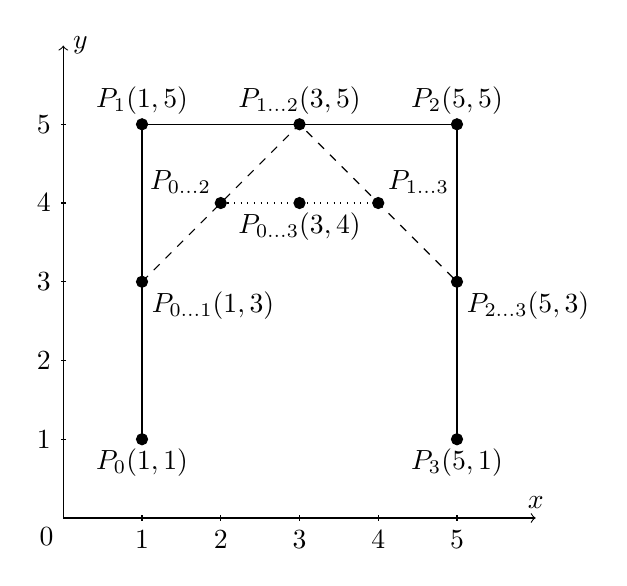
\begin{tikzpicture}[scale=1]
		% Coordinates
		\coordinate (P_0) at (1, 1);
		\coordinate (P_1) at (1, 5);
		\coordinate (P_2) at (5, 5);
		\coordinate (P_3) at (5, 1);
		
		\coordinate (P_0-1) at (1, 3);
		\coordinate (P_1-2) at (3, 5);
		\coordinate (P_2-3) at (5, 3);
		
		\coordinate (P_0-2) at (2, 4);
		\coordinate (P_1-3) at (4, 4);
		
		\coordinate (P_0-3) at (3, 4);
		
		% Draw X and Y axes
		\draw [->] (0,0) -- (0,6) node[align=left, right] {$y$};
		\draw [->] (0,0) -- (6,0) node[align=left, above] {$x$};
		\draw (0,0) node[anchor=north east,fill=white] {0};
		\foreach \x/\xtext in {1, 2, 3, 4, 5} 
			\draw (\x,1pt) -- (\x,-1pt) node[anchor=north,fill=white] {$\xtext$};
		\foreach \y/\ytext in {1, 2, 3, 4, 5} 
			\draw (1pt,\y) -- (-1pt,\y) node[anchor=east,fill=white] {$\ytext$};
			
		% First interpolation
		\draw (P_0) -- (P_1) -- (P_2) -- (P_3);
		
		\filldraw (P_0) circle (2pt) node[align=center, below] {$P_0(1,1)$};
		\filldraw (P_1) circle (2pt) node[align=center, above] {$P_1(1,5)$};
		\filldraw (P_2) circle (2pt) node[align=center, above] {$P_2(5,5)$};
		\filldraw (P_3) circle (2pt) node[align=center, below] {$P_3(5,1)$};
		
		% Second Interpolation
		\draw[dashed] (P_0-1) -- (P_1-2) -- (P_2-3);
		
		\filldraw (P_0-1) circle (2pt) node[align=center, below right] {$P_{0 \dotsc 1}(1,3)$};
		\filldraw (P_1-2) circle (2pt) node[align=center, above] {$P_{1 \dotsc 2}(3,5)$};
		\filldraw (P_2-3) circle (2pt) node[align=center, below right] {$P_{2 \dotsc 3}(5,3)$};
		
		% Third Interpolation
		\draw[dotted] (P_0-2) -- (P_1-3);
		
		\filldraw (P_0-2) circle (2pt) node[align=center, above left] {$P_{0 \dotsc 2}$};
		\filldraw (P_1-3) circle (2pt) node[align=center, above right] {$P_{1 \dotsc 3}$};
		
		% Interpolated Point
		\filldraw (P_0-3) circle (2pt) node[align=center, below] {$P_{0 \dotsc 3}(3, 4) $};
	\end{tikzpicture}
	\caption{Resulting point of the cubic interpolation}
\end{figure}

\end{example}

As such, the De Casteljau algorithm can be expressed as the following set of procedure:

\begin{enumerate}
\item Interpolate a set of points at $t \in [0, 1]$ for each of the consecutive pair of control points.
\item Repeat step \#1 with newly interpolated points, until a single point is left.
\end{enumerate}

Thus far, the B\'ezier curve has vaguely been mentioned, and its mathematical definition is yet unclear. However, this algorithm can be used to deduce the formal definition of a B\'ezier curve. Let $P_{a \dotsc b}(t)$ be a function that gives an interpolated point from a set of control points $P_a, P_{a+1}, P_{a+2},  \dotsc  , P_{b-1}, P_b$, where $a, b \in \mathbb Z_{\geq 0}$ and $a \geq b$. If $a = b$, $P_{a \dotsc b}(t) = P_a = P_b$. Next, let the control points of a B\'ezier curve be $P_0, P_1, P_2,  \dotsc  , P_{n-1}, P_{n}$. Performing a set of linear interpolation to consecutive pairs of control points at $t$ gives the following:

\begin{equation_nogap}\begin{aligned}
P_{0 \dotsc 1}(t)	& = P_0(1-t) + P_1t, \\
P_{1 \dotsc 2}(t)	& = P_1(1-t) + P_2t, \\
P_{2 \dotsc 3}(t)	& = P_2(1-t) + P_3t, \\
& \vdotswithin{=} \notag \\
P_{n-1 \dotsc n}(t)	& = P_{n-1}(1-t) + P_nt. \\
\\
\end{aligned}\end{equation_nogap}

The newly interpolated points can than be used to perform another set of interpolation.

\begin{equation_nogap}\begin{aligned}
P_{0 \dotsc 2}(t)	& = [P_{0 \dotsc 1}(t)](1-t) + [P_{1 \dotsc 2}(t)]t, \\
P_{1 \dotsc 3}(t)	& = [P_{1 \dotsc 2}(t)](1-t) + [P_{2 \dotsc 3}(t)]t, \\
P_{2 \dotsc 4}(t)	& = [P_{2 \dotsc 3}(t)](1-t) + [P_{3 \dotsc 4}(t)]t, \\
& \vdotswithin{=} \notag \\
P_{n-2 \dotsc n}(t)	& = [P_{n-2 \dotsc n-1}(t)](1-t) + [P_{n-1 \dotsc n}(t)]t. \\
\\
\end{aligned}\end{equation_nogap}

Substituting the interpolation functions with their definitions,

\begin{equation_nogap}\begin{aligned}
P_{0 \dotsc 2}(t)	& = [P_0(1-t)+P_1t](1-t) + [P_1(1-t)+P_2t]t, \\
P_{1 \dotsc 3}(t)	& = [P_1(1-t)+P_2t](1-t) + [P_2(1-t)+P_3t]t, \\
P_{2 \dotsc 4}(t)	& = [P_2(1-t)+P_3t](1-t) + [P_3(1-t)+P_4t]t, \\
& \vdotswithin{=} \notag \\
P_{n-2 \dotsc n}(t)	& = [P_{n-2}(1-t)+P_{n-1}t](1-t) + [P_{n-1}(1-t)+P_nt]t. \\
\\
\end{aligned}\end{equation_nogap}

Simplifying the equations above,

\begin{equation_nogap}\begin{aligned}
P_{0 \dotsc 2}(t)	& = P_0(1-t)^2 + 2P_1(1-t)t + P_2t^2, \\
P_{1 \dotsc 3}(t)	& = P_1(1-t)^2 + 2P_2(1-t)t + P_3t^2, \\
P_{2 \dotsc 4}(t)	& = P_2(1-t)^2 + 2P_3(1-t)t + P_4t^2, \\
& \vdotswithin{=} \notag \\
P_{n-2 \dotsc n}(t)	& = P_{n-2}(1-t)^2 + 2P_{n-1}(1-t)t + P_{n}t^2. \\
\\
\end{aligned}\end{equation_nogap}

\begin{absnopagebreak}
Following the same procedure of interpolating and simplifying yields the following:

\begin{equation_nogap}\begin{aligned}
P_{0 \dotsc 3}(t)	& = P_0(1-t)^3 + 3P_1(1-t)^2t + 3P_2(1-t)t^2 + P_3t^3, \\
P_{1 \dotsc 4}(t)	& = P_1(1-t)^3 + 3P_2(1-t)^2t + 3P_3(1-t)t^2 + P_4t^3, \\
P_{2 \dotsc 5}(t)	& = P_2(1-t)^3 + 3P_3(1-t)^2t + 3P_4(1-t)t^2 + P_5t^3, \\
& \vdotswithin{=} \notag \\
P_{n-3 \dotsc n}(t)	& = P_{n-3}(1-t)^3 + 3P_{n-2}(1-t)^2t + 3P_{n-1}(1-t)t^2 + P_{n}t^3. \\
\\
\end{aligned}\end{equation_nogap}
\end{absnopagebreak}

Repeating the same procedure again,

\begin{equation_nogap}\begin{aligned}
P_{0 \dotsc 4}(t)	& = P_0(1-t)^4 + 4P_1(1-t)^3t + 6P_2(1-t)^2t^2 + 4P_3(1-t)t^3 + P_4t^4, \\
P_{1 \dotsc 5}(t)	& = P_1(1-t)^4 + 4P_2(1-t)^3t + 6P_3(1-t)^2t^2 + 4P_4(1-t)t^3 + P_5t^4, \\
P_{2 \dotsc 6}(t)	& = P_2(1-t)^4 + 4P_3(1-t)^3t + 6P_4(1-t)^2t^2 + 4P_5(1-t)t^3 + P_6t^4, \\
& \vdotswithin{=} \notag \\
P_{n-4 \dotsc n}(t)	& = P_{n-4}(1-t)^4 + 4P_{n-3}(1-t)^3t + 6P_{n-2}(1-t)^2t^2 + 4P_{n-1}(1-t)t^3 + P_{n}t^4. \\
\\
\end{aligned}\end{equation_nogap}

A pattern that imitates binomial expansion of $((1-t) + t)^n$ emerges, along with the control points multiplied as coefficients of each terms. Continuing on a similar manner, the complete equation of interpolated B\'ezier curve is obtained.

\begin{multline}
P_{0 \dotsc n}(t) = 	P_0 \binom{n}{0}(1-t)^n + P_1 \binom{n}{1}(1-t)^{n-1}t + P_2 \binom{n}{2}(1-t)^{n-2}t^2 \\
				+ \dotsb + P_k \binom{n}{k}(1-t)^{n-k}t^k + \dotsb + P_{n-1} \binom{n}{n-1}(1-t)t^{n-1} + P_n \binom{n}{n}t^n,
\end{multline}

where $\binom{n}{k}$ is a binomial coefficient ($\binom{n}{k} = \frac{n!}{k!(n-k)!}$). Rewriting the equation above,

\begin{equation}
P_{0 \dotsc n}(t) = \sum_{i=0}^{n} {P_i \binom{n}{i} (1-t)^{n-i} t^i}.
\end{equation}

This, in fact, is the definition of the B\'ezier curve, which is written as $b_n(t)$ for curves with $n+1$ control points. As such, the mathematical development of B\'ezier curves from simple linear interpolation has been investigated so far. The following part of the essay will examine the properties of B\'eizer curves and why they allow is to be one of the most favoured method of describing curves in computer systems.

\section{Definition and Important Properties of B\'ezier Curves}

Thus far, we have investigated on the mathematical development of B\'ezier curves. However, before the attempt of approximating a cycloid can be made, the knowledge of definition and some important properties of B\'ezier curves must precede.

To reiterate the definition of B\'ezier curves,

\begin{definition}[\citeA{PRAUTZ:2013}]
\begin{equation}
b_n(t) = P_{0 \dotsc n} = \sum_{i=0}^{n} {P_i \binom{n}{i} (1-t)^{n-1} t^i}.
\end{equation}
\end{definition}

Although there are numerous properties of B\'ezier curves, the two most important ones are regarding their initial and terminal points, and the tangent at both points.

\begin{property} At $t=0$ and $t=1$, the interpolated points coincide with the first and last B\'ezier control points, respectively \cite{PRAUTZ:2013}.\end{property}

This will be useful when determining the location of the first an last control points of B\'ezier approximation based on the original curve.

\begin{property} The tangents at $t=0$ and $t=1$ pass through points $P_0$, $P_1$ and $P_{n-1}$, $P_n$, respectively \cite{PRAUTZ:2013}. \end{property}

This property is not so easy to realize without a visual intuition. As such, the next example graphically investigates this property to aid the understanding.

\begin{example}
Let $P_0 = (1,1), P_1 = (2, 3), P_2 = (3,3),$ and $P_3 = (4, 1)$. Plotting the control points and the B\'ezier curve yields the following:

\begin{figure}[H]
	\centering
	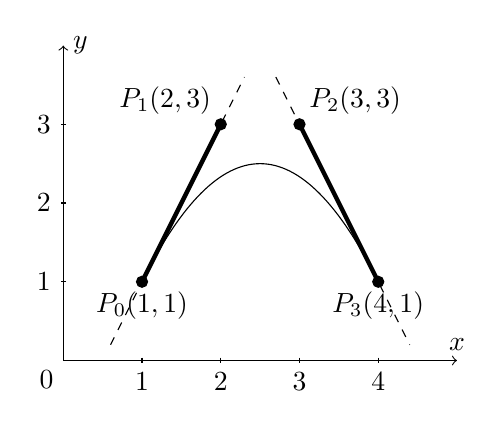
\begin{tikzpicture}[scale=1]
		% Coordinates
		\coordinate (P_0) at (1, 1);
		\coordinate (P_1) at (2, 3);
		\coordinate (P_2) at (3, 3);
		\coordinate (P_3) at (4, 1);
		
		% Draw X and Y axes
		\draw [->] (0,0) -- (0,4) node[align=left, right] {$y$};
		\draw [->] (0,0) -- (5,0) node[align=left, above] {$x$};
		\draw (0,0) node[anchor=north east,fill=white] {0};
		\foreach \x/\xtext in {1, 2, 3, 4} 
			\draw (\x,1pt) -- (\x,-1pt) node[anchor=north,fill=white] {$\xtext$};
		\foreach \y/\ytext in {1, 2, 3} 
			\draw (1pt,\y) -- (-1pt,\y) node[anchor=east,fill=white] {$\ytext$};
		
		% First interpolation
		\draw[ultra thick] (P_0) -- (P_1);
		\draw[ultra thick] (P_2) -- (P_3);
		
		\draw[thin, dashed] (0.6, 0.2) -- (2.3, 3.6);
		\draw[thin, dashed] (2.7, 3.6) -- (4.4, 0.2);
		
		\filldraw (P_0) circle (2pt) node[align=center, below] {$P_0(1,1)$};
		\filldraw (P_1) circle (2pt) node[align=center, above left] {$P_1(2,3)$};
		\filldraw (P_2) circle (2pt) node[align=center, above right] {$P_2(3,3)$};
		\filldraw (P_3) circle (2pt) node[align=center, below] {$P_3(4,1)$};
		
		\draw (P_0) .. controls (P_1) and (P_2) .. (P_3); 
	\end{tikzpicture}
	\caption{Tangent lines of a cubic B\'ezier curve}
\end{figure}

The tangents at the initial and terminal points ($t=0$ and $t=1$) of the curve show that they indeed pass through $P_0$, $P_1$ and $P_{n-1}$, $P_n$ ($P_2$, $P_3$ in this case), respectively.
\end{example}

By exploting the properties of the B\'ezier curve, we can now make different approaches to approximating a cycloid using a B\'ezier curve.

\section{Approximation of Cycloids}

As mentioned in the introduction of this essay, the B\'ezier curve is one of the most predominant means of representing curves and shapes on computer systems. As such, the topic of representing various kinds of curves, such as circles and ellipses, has been thoroughly investigated along with the improvement of computer graphics. However, because the B\'ezier curve is essentially a parametric polynomial curve, it cannot give an exact, mathematically equivalent representation of non-polynomial curves, such as circles, ellipses, and graphs of transcendental functions, such as that of sine and cosine function. However, there has been many successful attempts in approximating different kinds of curves, especially regarding the conic sections, such as an approximation given by Dokken et al (1989), which approximates a unit circle with a maximum error in radius of $2*10^{-6}$ with only 8 piecewise B\'ezier curves. However, after a thorough research, it was evident that there is no formal attempt of approximation done for cycloids using a B\'ezier curve. This came to me as a shock, because cycloids themselves are defined parametrically like B\'ezier curves, and it is also relatively easy to understand and manipulate. As such, I have determined to investigate on the extent in which a B\'ezier curve can be used to approximate a cycloid.

\textbf{Cycloid} is a parametric curve that is defined as following:

\begin{equation}
\begin{split}
x(\theta) & = \theta - \sin \theta, \\
y(\theta) & = 1 - \cos \theta.
\end{split}
\end{equation}

This is a curve that is generated by plotting the path in which a point on a circle that is rolling on a smooth, straight surface passes through. Graphically, it is illustrated by Fig. 6.1

\begin{figure}[H]
	\centering
	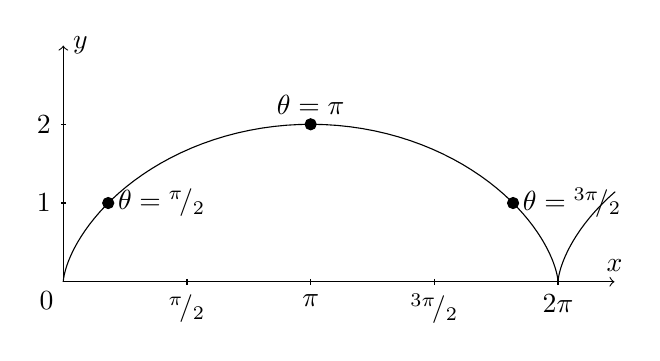
\begin{tikzpicture}[scale=1]
		% Draw X and Y axes
		\draw [->] (0,0) -- (0,3) node[align=left, right] {$y$};
		\draw [->] (0,0) -- (7,0) node[align=left, above] {$x$};
		\draw (0,0) node[anchor=north east,fill=white] {0};
		\draw (1.57079,1pt) -- (1.57079,-1pt) node[anchor=north,fill=white] {$\rfrac{\pi}{2}$};
		\draw (3.14159,1pt) -- (3.14159,-1pt) node[anchor=north,fill=white] {$\pi$};
		\draw (4.71238,1pt) -- (4.71238,-1pt) node[anchor=north,fill=white] {$\rfrac{3\pi}{2}$};
		\draw (6.28318,1pt) -- (6.28318,-1pt) node[anchor=north,fill=white] {$2\pi$};
		\foreach \y/\ytext in {1, 2} 
			\draw (1pt,\y) -- (-1pt,\y) node[anchor=east,fill=white] {$\ytext$};
			
		\draw[domain=0:8, samples=100] plot ({\x - sin(\x r)},{1 - cos(\x r)});
		
		\filldraw (0.57079, 1) circle (2pt) node[align=center, right] {$\theta = \rfrac{\pi}{2}$};
		\filldraw (3.14159, 2) circle (2pt) node[align=center, above] {$\theta = \pi$};
		\filldraw (5.71238, 1) circle (2pt) node[align=center, right] {$\theta = \rfrac{3\pi}{2}$};
	\end{tikzpicture}
	\caption{An arc of cycloid}
\end{figure}

Because this curve repeats infinitely, approximating one arc will yield a complete repeatable approximation of the curve. Moreover, since an arc of a cycloid is symmetrical at $\theta = \pi$, we only need to approximate $\theta \in [0, \pi]$ section of the arc, which is illustrated in Fig. 6.2.

\begin{figure}[H]
	\centering
	\begin{tikzpicture}[scale=1]
		% Draw X and Y axes
		\draw [->] (0,0) -- (0,3) node[align=left, right] {$y$};
		\draw [->] (0,0) -- (4,0) node[align=left, above] {$x$};
		\draw (0,0) node[anchor=north east,fill=white] {0};
		\draw (1.57079,1pt) -- (1.57079,-1pt) node[anchor=north,fill=white] {$\rfrac{\pi}{2}$};
		\draw (3.14159,1pt) -- (3.14159,-1pt) node[anchor=north,fill=white] {$\pi$};
		\foreach \y/\ytext in {1, 2} 
			\draw (1pt,\y) -- (-1pt,\y) node[anchor=east,fill=white] {$\ytext$};
			
		\draw[domain=0:3.14159, samples=40] plot ({\x - sin(\x r)},{1 - cos(\x r)});
	\end{tikzpicture}
	\caption{Section of cycloid for $\theta \in [0, \pi]$}
\end{figure}

In order to make the comparison between the cycloid and the B\'ezier approximation easier, the cycloid can be redefined as following with respect to variable $t$ so that the arc in Fig 6.2 will be constructed for $t \in [0, 1]$.

\begin{equation}
\begin{split}
x(t) & = \pi t - \sin \pi t, \\
y(t) & = 1 - \cos \pi t.
\end{split}
\end{equation}

The three methods of approximation that will be investigated in this paper will be based on the Maclaurin polynomial, approximation of unit circle given by \citeA{DOKKEN:1990}, and numerical analysis. Although these are not the only methods of approximating a non-polynomial curve with a B\'ezier curve, they will allow a through comparison and holistic judgement of B\'ezier curve as a means of approximation to be made.

In all three approximations, cubic B\'ezier curves will be used, because they are most commonly used in most of the popular computer-aided design (CAD) softwares, such as Photoshop \cite{FULLER:2007} and GIMP \cite{GOELKER:2007}, portraying them as being much more practical than curves of other degrees.

When evaluating the approximation, two approaches may be used: Extent of tangential approximation at initial and terminal points, and numerical error analysis.

In Fig. 6.2, it shows that the initial and terminal points of the cycloid are $(0,0)$ and $(\pi, 2)$, respectively. Moreover, the calculating the derivatives at $t=0$ and $t=1$ also shows that it has vertical and horizontal tangents at the initial and terminal points, respectively.

\begin{equation_nogap}\begin{aligned}
\frac{dy}{dx} 	&= \frac{\frac{d}{dt}(1-\cos(\pi t)}{\frac{d}{dt}(\pi t - \sin(\pi t)} \\
			&= \frac{\pi\sin(\pi t)}{\pi - \pi\cos(\pi t)}. \\
\\
\end{aligned}\end{equation_nogap}

By L'H\^opital's rule of indeterminate forms, at the initial point $t=0$,

\begin{equation_nogap}\begin{aligned}
\frac{dy}{dx}|_{t=0} 	&= \lim_{t\to 0^+} \frac{\pi\sin(\pi t)}{\pi - \pi\cos(\pi t)} \\ % Explain why it is one-sided limit
				&= \lim_{t\to 0^+} \frac{\pi^2\cos(\pi t)}{\pi^2\sin(\pi t)} \\
				&= + \infty \text{ (Vertical tangent)} \\
\\
\end{aligned}\end{equation_nogap}

At the terminal point $t=1$,

\begin{equation_nogap}\begin{aligned}
\frac{dy}{dx}|_{t=1} 	&= \frac{\pi\sin(\pi * 0)}{\pi - \pi\cos(\pi * 0)} \\ % Explain why it is one-sided limit
				&= 0 \text{ (Horizontal tangent)}. \\
\\
\end{aligned}\end{equation_nogap}

As such, assessing if the approximated curve tangentially coincides with the original cycloid will allow us to assess the quality of the approximation to some extent.

For the numerical analysis, we must define a error function that will yield numerical values for the accuracies of different approximations, which will allow a reasoned comparison to be made. Using the Pythagoras theorem, the Euclidean distance between the cycloid and the B\'ezier approximation at $t \in [0,1]$ can be computed, as following:

\begin{equation}
\epsilon (t) = \sqrt{(x(t) - b_x(t))^2 + (y(t) - b_y(t))^2},
\end{equation}

where $x(t)$ and $y(t)$ are the $x$ and $y$ components of the parametric equations of a cycloid, and $b_x(t)$ and $x$ and $y$ components of the B\'ezier approximation. Thus, taking $\max\limits_{t \in [0, 1]} \epsilon (t)$, we can evaluate the maximum error of the approximation, obtaining another way to assess the quality of the approximation to some extent.

%However, a low maximum error does not necessarily guarantee the approximation to appear similar to the original cycloid. The following example shows why this is the case.
%
%\begin{example} By setting B\'ezier control points $P_0=(0, 0), P_1=(0, 0.7), P_2=(1.28, 2), P_3=(\pi,2)$, a seemingly excellent approximation of a cycloid is made, as shown in Fig. 6.3.
%
%\begin{figure}[H]
%	\centering
%	\begin{tikzpicture}[scale=1]
%		% Draw X and Y axes
%		\draw [->] (0,0) -- (0,3) node[align=left, right] {$y$};
%		\draw [->] (0,0) -- (5,0) node[align=left, above] {$x$};
%		\draw (0,0) node[anchor=north east,fill=white] {0};
%		\foreach \x/\xtext in {1, 2, 3, 4} 
%			\draw (\x, 1pt) -- (\x, -1pt) node[anchor=north,fill=white] {$\xtext$};
%		\foreach \y/\ytext in {1, 2} 
%			\draw (1pt,\y) -- (-1pt,\y) node[anchor=east,fill=white] {$\ytext$};
%			
%		\draw (0,0) .. controls (0, 0.7) and (1.28, 2) .. (3.14, 2);
%	\end{tikzpicture}
%	\caption{Empirical approximation of a cycloid}
%\end{figure}
%
%However, plotting the error function $\epsilon$ of this graph exposes its weakness, as shown in Fig. 6.4.
%
%\begin{figure}[H]
%	\centering
%	\begin{tikzpicture}
%		\begin{axis}[xlabel=$t$, ylabel=$\epsilon(t)$, domain=0:1.0, samples=100]
%			\addplot[black] {sqrt((\bezier(x, 0, 0, 1.28, 3.14) - (3.14*x - sin(deg(3.14*x))))^2 + (\bezier(x, 0, 0.7, 2, 2) - (1 - cos(deg(3.14*x))))^2)};%
%		\end{axis}
%	\end{tikzpicture}
%	\caption{Error of the Approximation}
%\end{figure}
%
%The graph shows that the maximum error of this approximation is 0.412 at $t=0.421$. Considering how the maximum error \citeA{DOKKEN:1990} was able to give an approximation of a quarter unit circle with a maximum error in radius of $1.4*10^{-4}$, this approximation is clearly not as good as it first appears. The reason of this is because, although the approximated curve as a whole looks like a good approximation, the individual interpolated points at certain value of $t$ is quite far from the original cycloid. For instance, at $t=0.421$, the point on the original curve and the interpolated point from the B\'ezier approximation is shown in Fig. 6.5.
%
%\begin{figure}[H]
%	\centering
%	\begin{tikzpicture}[scale=1.4]
%		% Draw X and Y axes
%		\draw [->] (0,0) -- (0,3) node[align=left, right] {$y$};
%		\draw [->] (0,0) -- (5,0) node[align=left, above] {$x$};
%		\draw (0,0) node[anchor=north east,fill=white] {0};
%		\foreach \x/\xtext in {1, 2, 3, 4} 
%			\draw (\x, 1pt) -- (\x, -1pt) node[anchor=north,fill=white] {$\xtext$};
%		\foreach \y/\ytext in {1, 2} 
%			\draw (1pt,\y) -- (-1pt,\y) node[anchor=east,fill=white] {$\ytext$};
%			
%		\draw (0,0) .. controls (0, 0.7) and (1.28, 2) .. (3.14, 2);
%		
%		\filldraw (0.353, 0.754) circle (2pt) node[align=center, below right] {$Original$};
%		\filldraw (0.628, 1.061) circle (2pt) node[align=center, above right] {$Approximation$};
%	\end{tikzpicture}
%	\caption{Interpolated points at $t=0.421$}
%\end{figure}
%
%\end{example}
%
%This disparity between the appearance and the actual mathematical quality of approximation allow us to understand the results of the approximation from numerical analysis later in this essay.

\subsection{Maclaurin Polynomial}

A Maclaurin polynomial $P_n(x)$ approximates a function $f(n)$ with order $n$ as following:

\begin{equation}
f(x) \approx P_n(x) = f(0) + f'(0)x + \frac{f''(0)}{2!}x^2 + \frac{f'''(0)}{3!} + \dotsc + \frac{f^{(n)}(0)}{n!}
\end{equation}

Using the Maclaurin polynomial, the parametric equations of cycloid can be approximated. Because a cubic B\'ezier curve is used, a Maclaurin polynomial with order of 3 must be used.

\begin{equation_nogap}\begin{aligned}
x(t) 	& \approx x(0) + x'(0)t + \frac{x''(0)}{2!}t^2 + \frac{x'''(0)}{3!}t^3 \\
	& = (\pi t - sin \pi t)|_{t=0} + (\pi - \pi cos \pi t)|_{t=0} + \frac{(\pi^2 sin \pi t)|_{t=0}}{2}t^2 + \frac{(\pi^3 cos \pi t)|_{t=0}}{6}t^3 \\
	& = \frac{{\pi^3}}{6}t^3  \\
y(t)	& \approx y(0) + y'(0)t + \frac{y''(0)}{2!}t^2 + \frac{y'''(0)}{3!}t^3 \\
	& = (1 - cos \pi t)\_{t=0} + (\pi sin \pi t)|_{t=0} t + \frac{(\pi^2 cos \pi t)|_{t=0}}{2}t^2 + \frac{(-\pi^3 sin \pi t)|_{t=0}}{6}t^3 \\
	& = \frac{\pi^2}{2}t^2 \\
	\\
\end{aligned}\end{equation_nogap}

Let $b(t)$ be a cubic B\'ezier approximation of cycloid. To rearrange the Maclaurin polynomial into a B\'ezier form, we must first expand and simplify the definition of B\'ezier curve into a polynomial in terms of $t$.

\begin{equation_nogap}\begin{aligned}
b(t) 	& = \sum_{i=0}^{3} {P_i \binom{3}{i} (1-t)^{3-i} t^i} \\
	& = P_0(1-t)^3 + 3P_1(1-t)^2t + 3P_2(1-t)t^2 + P_3t^3 \\
	& = P_0(1-3t+3t^2+t^3) + 3P_1(t-2t^2+t^3) + 3P_2(t^2-t^3) + P_3t^3 \\
	& = P_0 - 3P_0t + 3P_0t^2 - P_0t^3 + 3P_1t - 6P_1t^2 + 3P_1t^3 + 3P_2t^2 - 3P_2t^3 + P_3t^3 \\
	&= P_0 + 3(P_1 - P_0)t + 3(P_2 - 2P_1 + P_0)t^2 + (P_3 - 3P_2 + 3P_1 - P_0)t^3 \\
	\\
\end{aligned}\end{equation_nogap}

Since

\begin{equation_nogap}\begin{aligned}
b_x(t) \approx x(t) \approx \frac{\pi^3}{6}t^3 \text{\qquad and \qquad} b_y(t)  \approx y(t) \approx \frac{\pi^2}{2}t^2, \\
\\
\end{aligned}\end{equation_nogap}

we can equate the coefficients of each terms of $b(t)$ with those of Maclaurin approximations of $x(t)$ and $y(t)$ to find the control points. Firstly, for the $x$ component of the control points, we obtain 4 simultaneous equations as following:

\begin{equation_nogap}\begin{aligned}
P_{0,x} &= 0, \\
3(P_{1,x} - P_{0,x}) &= 0, \\
3(P_{2,x} - 2P_{1,x} + P_{0,x}) &= 0, \\
P_{3,x} - 3P_{2,x} + 3P_{1,x} - P_{0,x} &= \frac{\pi^3}{6}. \\
\\
\end{aligned}\end{equation_nogap}

Solving the simultaneous equations above yields

\begin{equation_nogap}\begin{aligned}
\therefore P_{0,x} &= 0, \\
\therefore P_{1,x} &= 0, \\
\therefore P_{2,x} &= 0, \\
\therefore P_{3,x} &= \frac{\pi^3}{6}. \\
\\
\end{aligned}\end{equation_nogap}

Then, for the y component of the control points, we have another 4 simultaneous equations as following:

\begin{equation_nogap}\begin{aligned}
P_{0,y} &= 0, \\
3(P_{1,y} - P_{0,y}) &= 0, \\
3(P_{2,y} - 2P_{1,y} + P_{0,y}) &= \frac{\pi^2}{2}, \\
P_{3,y} - 3P_{2,y} + 3P_{1,y} - P_{0,y} &= 0. \\
\\
\end{aligned}\end{equation_nogap}

Solving the simultaneous equations above yields

\begin{equation_nogap}\begin{aligned}
\therefore P_{0,y} &= 0, \\
\therefore P_{1,y} &= 0, \\
\therefore P_{2,y} &= \frac{\pi^2}{6}, \\
\therefore P_{3,y} &= \frac{\pi^2}{2}. \\
\\
\end{aligned}\end{equation_nogap}

As such, the cubic Maclaurin approximation of cycloid yields the following B\'ezier control points:

\begin{equation_nogap}\begin{aligned}
P_0 = \begin{bmatrix}0 \\ 0\end{bmatrix}, \kern 3em P_1 = \begin{bmatrix}0 \\ 0\end{bmatrix} \\
P_2 = \begin{bmatrix}0 \\ \frac{\pi^2}{6} \end{bmatrix}, \kern 3em P_3 = \begin{bmatrix} \frac{\pi^3}{6} \\ \frac{\pi^2}{2} \end{bmatrix} \\
\\
\end{aligned}\end{equation_nogap}

This approximation is shown in Fig. 6.6.

\begin{figure}[H]
	\centering
	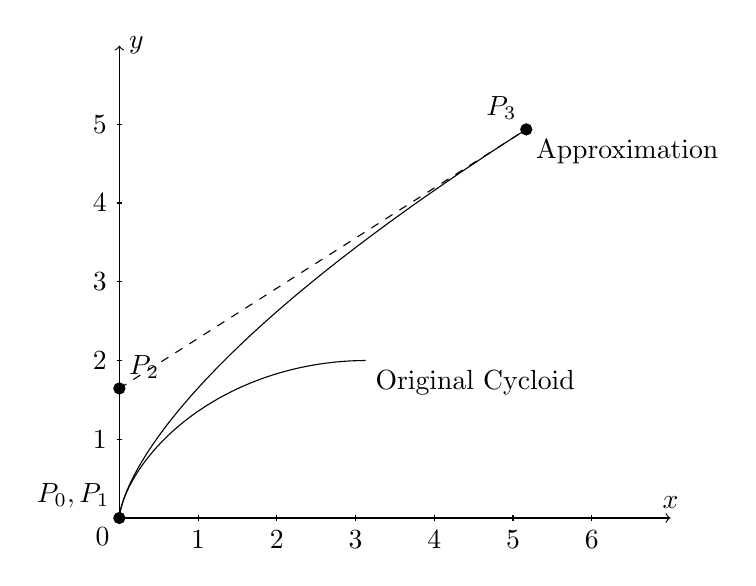
\begin{tikzpicture}[scale=1]
		% Draw X and Y axes
		\draw [->] (0,0) -- (0,6) node[align=left, right] {$y$};
		\draw [->] (0,0) -- (7,0) node[align=left, above] {$x$};
		\draw (0,0) node[anchor=north east,fill=white] {0};
		\foreach \x/\xtext in {1, 2, 3, 4, 5, 6} 
			\draw (\x, 1pt) -- (\x, -1pt) node[anchor=north,fill=white] {$\xtext$};
		\foreach \y/\ytext in {1, 2, 3, 4, 5} 
			\draw (1pt,\y) -- (-1pt,\y) node[anchor=east,fill=white] {$\ytext$};
			
		\draw[domain=0:1, samples=100] plot ({(3.14)*\x - sin((3.14)*\x r)},{1 - cos((3.14)*\x r)}) node[align=center, below right] {Original Cycloid};
		\draw (0,0) .. controls (0, 0) and (0, 1.645) .. (5.168, 4.935) node[align=center, below right] {Approximation};
		
		\filldraw (0, 0) circle (2pt) node[align=center, above left] {$P_0, P_1$};
		\filldraw (0, 1.645) circle (2pt) node[align=center, above right] {$P_2$};
		\filldraw (5.168, 4.935) circle (2pt) node[align=center, above left] {$P_3$};
		
		\draw[dashed] (0, 0) -- (0, 1.645);
		\draw[dashed] (0, 1.645) -- (5.168, 4.935);
	\end{tikzpicture}
	\caption{Approximation using Maclaurin series}
\end{figure}

This shws that the approximated B\'ezier curve will tangentially meet the original cycloid at $t=0$, satisfying the boundary condition at the initial point. However, as the curves approach their terminal points, the error in approximation becomes very large. Also, the B\'ezier curve does not coincide with the curve nor have same slope of tangent at $t=1$.

When error function of this approximation is plotted on a graph, it is clear that the maximum error occurs at $t=1$, as shown in Fig. 6.7.

\begin{figure}[H]
	\centering
	\begin{tikzpicture}
		\begin{axis}[xlabel=$t$, ylabel=$\epsilon(t)$, domain=0:1.0, samples=100]
			\addplot[black] {sqrt((\bezier(x, 0, 0, 0, 5.168) - (3.14*x - sin(deg(3.14*x))))^2 + (\bezier(x, 0, 0, 1.645, 4.935) - (1 - cos(deg(3.14*x))))^2)};%
		\end{axis}
	\end{tikzpicture}
	\caption{Error of the approximation using Maclaurin polynomial}
\end{figure}

A computation of error function at $t=1$ yields that the maximum error is approximately 3.566.

\subsection{Approximation of Trigonometric Function by Dokken et al. (1990)}

Dokken et al gives an excellent B\'ezier approximation of a unit circle in their paper "Good approximation of circles by curvature-continuous Bezier curves" from 1990. In fact, they were able to approximate a quarter sector with maximum error in radius of $1.4*10^{-4}$, which is a maximum of 0.014\% error from the original circle. By taking the $x$ and $y$ components of their B\'ezier approximation, we can obtain a good approximation of cosine and sine functions, respectively.

\citeA{DOKKEN:1990} proved that a cubic B\'ezier curve with following control points has a maximum radial error of $\frac{1}{27}$ from a unit semicircle.

\begin{equation_nogap}\begin{aligned}
P_0 & = \begin{bmatrix}1 \\ 0\end{bmatrix}, \kern 3em &P_1 & = \begin{bmatrix}1 \\ 0\end{bmatrix} + L\begin{bmatrix}0 \\ 1\end{bmatrix}, \\
P_2 & = \begin{bmatrix}\cos \pi \\ \sin \pi \end{bmatrix} - L\begin{bmatrix}-\sin \pi \\ \cos \pi \end{bmatrix}, \kern 3em &P_3 & = \begin{bmatrix}\cos \pi \\ \sin \pi \end{bmatrix}, \\
\\
\end{aligned}\end{equation_nogap}

where $L = \frac{4}{3}\tan\frac{\pi}{4} = \frac{4}{3}$. Substituting the value of L and simplifying yields

\begin{equation_nogap}\begin{aligned}
P_0 & = \begin{bmatrix}1 \\ 0\end{bmatrix}, \kern 3em &P_1 & = \begin{bmatrix}1 \\ \frac{4}{3}\end{bmatrix}, \\
P_2 & = \begin{bmatrix} -1 \\ \frac{4}{3} \end{bmatrix}, \kern 3em &P_3 & = \begin{bmatrix} -1 \\ 0 \end{bmatrix}, \\
\\
\end{aligned}\end{equation_nogap}

As such, a cubic B\'ezier approximation of a unit semicircle is

\begin{equation_nogap}\begin{aligned}
x(t) (= \cos(\pi t)) &\approx (1-t)^3 + 3(1-t)^2t - 3(1-t)t^2 - t^3, \\
y(t) (= \sin(\pi t)) &\approx 4(1-t)^2t + 4(1-t)t^2. \\
\\
\end{aligned}\end{equation_nogap}

By substituting the $x$ and $y$ components of the above B\'ezier curve as approximations of trigonometric functions in the parametric equations of a cycloid, an approximation of a cycloid can be obtained as following.

\begin{equation_nogap}\begin{aligned}
x(t) 	&= \pi t - \sin (\pi t) \\
	&\approx \pi t - (4(1-t)^2t + 4(1-t)t^2) \\ 
	&= \pi t - 4(t-2t^2+t^3) - 4(t^2 - t^3) \\
	&= \pi t - 4t + 8t^2 - 4t^3 - 4t^2 + 4^3 \\
	&= (\pi - 4)t + 4t^2. \\
	\\
\end{aligned}\end{equation_nogap}

\begin{equation_nogap}\begin{aligned}
y(t) 	&= 1 - \cos(\pi t) \\ 
	&\approx 1 - ((1-t)^3 + 3(1-t)^2t - 3(1-t)t^2 - t^3) \\
	&= 1 - (1-t)^3 - 3(1-t)^2t + 3(1-t)t^2 + t^3 \\
	&= 1 - (1-3t+3t^2-t^3) - 3(t-2t^2+t^3) + 3(t^2 - t^3) + t^3 \\
	&= 1 - 1 + 3t - 3t^2 + t^3 - 3t + 6t^2 - 3t^3 + 3t^2 - 3t^3 + t^3\\
	&= 6t^2 - 4t^3. \\
	\\
\end{aligned}\end{equation_nogap}

In order to put this parametric equations into a B\'ezier form, we will follow the similar process of simplifying the equation of a B\'ezier curve with respect to $t$ and equating the coefficients.

Since

\begin{equation_nogap}\begin{aligned}
b(t) 	&= \sum_{i=0}^{3} {P_i \binom{3}{i} (1-t)^{3-i} t^i}. \\ 
	&= P_0(1-3t+3t^2+t^3) + 3P_1(t-2t^2+t^3) + 3P_2(t^2-t^3) + P_3t^3 \\ 
	&= P_0 + 3(P_1-P_0)t + 3(P_2-2P_1+P_0)t^2 + (P_3-3P_2+3P_1-P_0)t^3,\\
\\
\end{aligned}\end{equation_nogap}

the following 4 simultaneous equations for the $x$ component of the control points can be produced by equating the coefficients with that of the approximation above.

\begin{equation_nogap}\begin{aligned}
P_{0,x} &= 0, \\
3(P_{1,x} - P_{0,x}) &= \pi -4, \\
3(P_{2,x} - 2P_{1,x} + P_{0,x}) &= 4, \\
P_{3,x}-3P_{2,x}+3P_{1,x}-P_{0,x} &= 0, \\
\\
\end{aligned}\end{equation_nogap}

Solving the simultaneous equations yields

\begin{equation_nogap}\begin{aligned}
\therefore P_{0,x} &= 0, \\
\therefore P_{1,x} &= \frac{\pi -4}{3}, \\
\therefore P_{2,x} &= \frac{2\pi -4}{3}, \\
\therefore P_{3,x} &= \pi, \\
\\
\end{aligned}\end{equation_nogap}

Similarly, another set of 4 simultaneous equations can be produced for the $y$ component of the control points.

\begin{equation_nogap}\begin{aligned}
P_{0,x} &= 0, \\
3(P_{1,x} - P_{0,x}) &= 0, \\
3(P_{2,x} - 2P_{1,x} + P_{0,x}) &= 6, \\
P_{3,x}-3P_{2,x}+3P_{1,x}-P_{0,x} &= -4, \\
\\
\end{aligned}\end{equation_nogap}

Solving the simultaneous equations yields

\begin{equation_nogap}\begin{aligned}
\therefore P_{0,x} &= 0, \\
\therefore P_{1,x} &= 0, \\
\therefore P_{2,x} &= 2, \\
\therefore P_{3,x} &= 2, \\
\\
\end{aligned}\end{equation_nogap}

As such, the control points of the cubic B\'ezier approximation of cycloid using Dokken et al.'s approximation of unit semicircle are

\begin{equation_nogap}\begin{aligned}
P_0 & = \begin{bmatrix}0 \\ 0\end{bmatrix}, \kern 3em &P_1 & = \begin{bmatrix}\frac{\pi - 4}{3} \\ 0\end{bmatrix}, \\
P_2 & = \begin{bmatrix} \frac{2\pi - 4}{3} \\ 2 \end{bmatrix}, \kern 3em &P_3 & = \begin{bmatrix} \pi \\ 2 \end{bmatrix}, \\
\\
\end{aligned}\end{equation_nogap}

Graphing the approximation and its error yields the following:

\begin{figure}[H]
	\centering
	\begin{tikzpicture}[scale=1.3]
		% Draw X and Y axes
		\draw [->] (0,0) -- (0,3) node[align=left, right] {$y$};
		\draw [->] (0,0) -- (5,0) node[align=left, above] {$x$};
		\draw (0,0) node[anchor=north east,fill=white] {0};
		\foreach \x/\xtext in {1, 2, 3, 4} 
			\draw (\x, 1pt) -- (\x, -1pt) node[anchor=north,fill=white] {$\xtext$};
		\foreach \y/\ytext in {1, 2} 
			\draw (1pt,\y) -- (-1pt,\y) node[anchor=east,fill=white] {$\ytext$};
			
		\draw (0,0) .. controls (-0.28613578, 0) and (0.761061769, 2) .. (3.14159265, 2);
	\end{tikzpicture}
	\caption{B\'ezier approximation using unit semicircle approximation by Dokken et al. (1990)}
\end{figure}

\begin{figure}[H]
	\centering
	\begin{tikzpicture}
		\begin{axis}[xlabel=$t$, ylabel=$\epsilon(t)$, domain=0:1.0, samples=150]
			\addplot[black] {sqrt((\bezier(x, 0, (pi-4)/3, (2*pi-4)/3, pi) - (3.14*x - sin(deg(pi*x))))^2 + (\bezier(x, 0, 0, 2, 2) - (1 - cos(deg(pi*x))))^2)};%
		\end{axis}
	\end{tikzpicture}
	\caption{Error of the approximation}
\end{figure}

Fig 6.9 shows that the maximum error of the approximation is 0.0575, which occurs twice at $t=0.157$ and $t=0.843$. Compared to the previous approximation, this is clearly much closer to the original curve. Moreover, it coincides with the original curve at $t=0$ and $t=1$, and the slope of the tengent line at $t=1$ is 0 (horizontal), which is equal to that of the original curve. However, at $t=0$, the tangent lines of the two curves are perpendicular to each other. The cycloid has a vertical tangent, whereas, because the control points $P_0, P_1$ form a flat horizontal line, the B\'ezier approximation has a horizontal curve. This is shown more clearly in Fig. 6.10.

\begin{figure}[H]
	\centering
	\begin{tikzpicture}
		\begin{axis}[xlabel=$x$, ylabel=$y$, domain=0:0.3, samples=100]
			\addplot[black, ultra thick] ({\bezier(x, 0, (pi-4)/3, (2*pi-4)/3, pi)}, {\bezier(x, 0, 0, 2, 2)});
			\addlegendentry{$Approximation$}?
			
			\addplot[black] ({pi*x - sin(deg(pi*x))}, {1-cos(deg(pi*x))});
			\addlegendentry{$Original$}?
		\end{axis}
	\end{tikzpicture}
	\caption{Error of the approximation}
\end{figure}

As such, this approximation fails to tangentially coincide the original cycloid at $t=0$, slightly harming its accuracy.

%Calculating the derivative of the B\'ezier curve at $t=0$ also reveals that its tangent is perpendicular to that of the original cycloid.
%
%\begin{equation_nogap}\begin{aligned}
%\frac{dy}{dx}_{B\acute ezier} 	&= \frac{\frac{d}{dt}{P_{0,y}(1-t)^3 + 3P_{1,y}(1-t)^2t + 3P_{2,y}(1-t)t^2 + P_{3,y}t^3}}{\frac{d}{dt}{P_{0,x}(1-t)^3 + 3P_{1,x}(1-t)^2t + 3P_{2,x}(1-t)t^2 + P_{3,x}t^3}} \\ 
%						&= \frac{\frac{d}{dt}{P_{0,y}(1-3t+3t^2+t^3) + 3P_{1,y}(t-2t^2+t^3) + 3P_{2,y}(t^2-t^3) + P_{3,y}t^3}}{\frac{d}{dt}{P_{0,x}(1-3t+3t^2+t^3) + 3P_{1,x}(t-2t^2+t^3) + 3P_{2,x}(t^2-t^3) + P_{3,x}t^3}} \\
%						&= \frac{\frac{d}{dt}{P_{0,y}(-3+6t-3t^2) + 3P_{1,y}(1-4t+3t^2) + 3P_{2,y}(2t-3t^2) + 3P_{3,y}t^2}}{\frac{d}{dt}{P_{0,x}(-3+6t-3t^2) + 3P_{1,x}(1-4t+3t^2) + 3P_{2,x}(2t-3t^2) + 3P_{3,x}t^2}}. \\
%\\
%\end{aligned}\end{equation_nogap}
%
%Substituting $t=0$,
%
%\frac{dy}{dx}_{B\acute ezier}

\subsection{Iterative Numerical Approximation}

With the help of numerical analysis using a computer, a very close approximation can be made. However, in order to do so, we must exploit the properties of B\'ezier curves.

We know that the initial and terminal control points ($P_0$ and $P_3$, respectively) coincides with the interpolated point of the B\'ezier curve will be at $t=0$ and $t=1$, respectively. Moreover, the second and third control points ($P_1$ and $P_2$, respectively) will lay on the tangent of the original curve at $t=0$ and $t=1$ if the approximation were to tangentially coincide with the original curve at the initial and terminal points. Graphically, this can be represented as shown in Fig. 6.11.

\begin{figure}[H]
	\centering
	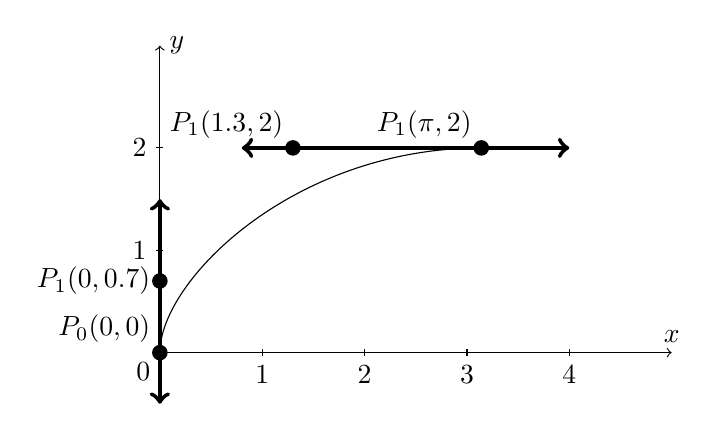
\begin{tikzpicture}[scale=1.3]
		% Draw X and Y axes
		\draw [->] (0,0) -- (0,3) node[align=left, right] {$y$};
		\draw [->] (0,0) -- (5,0) node[align=left, above] {$x$};
		\draw (0,0) node[anchor=north east,fill=white] {0};
		\foreach \x/\xtext in {1, 2, 3, 4} 
			\draw (\x, 1pt) -- (\x, -1pt) node[anchor=north,fill=white] {$\xtext$};
		\foreach \y/\ytext in {1, 2} 
			\draw (1pt,\y) -- (-1pt,\y) node[anchor=east,fill=white] {$\ytext$};
			
		\draw (0,0) .. controls (0, 0.7) and (1.3, 2) .. (3.14, 2);
		\draw[ultra thick, <->] (0,-0.5) -- (0, 1.5);
		\draw[ultra thick, <->] (0.8,2) -- (4, 2);
		
		\filldraw (0, 0) circle (2pt) node[align=center, above left] {$P_0(0,0)$};
		\filldraw (0, 0.7) circle (2pt) node[align=center, left] {$P_1(0,0.7)$};
		\filldraw (1.3, 2) circle (2pt) node[align=center, above left] {$P_1(1.3, 2)$};
		\filldraw (3.14, 2) circle (2pt) node[align=center, above left] {$P_1(\pi,2)$};
	\end{tikzpicture}
	\caption{Possible arrangement of the control points}
\end{figure}

As such, the control points will be as following:

\begin{equation_nogap}\begin{aligned}
P_0 & = \begin{bmatrix}0 \\ 0\end{bmatrix}, \kern 3em &P_1 & = \begin{bmatrix}0 \\ 0\end{bmatrix} + \begin{bmatrix}0 \\ u\end{bmatrix}, \\
P_2 & = \begin{bmatrix}\pi \\ 2\end{bmatrix} - \begin{bmatrix}v \\ 0\end{bmatrix}, \kern 3em &P_3 & = \begin{bmatrix} \pi \\ 2 \end{bmatrix}, \\
\\
\end{aligned}\end{equation_nogap}

where $u, v \in \mathbb{R}^+$. As such, finding values of $u$ and $v$ that will minimize the maximum error $\max\limits_{t \in [0, 1]} \epsilon (t)$ will give a close approximation of a cycloid with a cubic B\'ezier curve that fits the criteria of initial and terminal points discussed before.

Let $\zeta (u, v)$ be a function that gives that maximum error of B\'ezier approximation for given values $u$ and $v$, or

\begin{equation}
\zeta (u, v) = \max\limits_{t \in [0, 1]} \epsilon (t).
\end{equation}

As such, $\argmin\limits_{u, v} (\zeta (u, v))$ will yield values $u, v$ that will give the best possible approximation. Graphing $\zeta (u, v)$ using GNU Octave yields the following:

\begin{figure}[H]
	\centering
	\includegraphics[width=13cm]{numerical_analysis_graph}
	\caption{Plot of $u, v \in [-4, 4]$ and $\zeta (u, v)$}
\end{figure}

Using GNU Octave, $\argmin\limits_{u, v} (\zeta (u, v))$ is approximated iteratively, with initial domains of $u \in [0, 2]$ and $v \in [1, 3]$, in which each iteration subdivides the initial interval into 10, finds the minimum, and finds the minimum around the $u, v$ discovered from previous iteration with a domain of $\pm$ the previous interval. The 10 subdivision is chosen because it is enough to ensure that the iteration will converge into the minimum within the initial domains, which can be deduced by examining Fig. 6.12. For the specific programming code, see Appendix A.

After 10 iteration, the approximation converged to $u=0.000988889$ and $v=2.50477$ with $\zeta (u, v) = 0.0809535$. As such, the control points of the B\'ezier approximation are

\begin{equation_nogap}\begin{aligned}
P_0 & = \begin{bmatrix}0 \\ 0\end{bmatrix}, \kern 3em &P_1 & = \begin{bmatrix}0 \\ 0.000988889\end{bmatrix}, \\
P_2 & = \begin{bmatrix}\pi - 2.50477 \\ 2\end{bmatrix}, \kern 3em &P_3 & = \begin{bmatrix} \pi \\ 2 \end{bmatrix}. \\
\\
\end{aligned}\end{equation_nogap}

Graphing the B\'ezier approximation yields the following:

\begin{figure}[H]
	\centering
	\begin{tikzpicture}[scale=1.3]
		% Draw X and Y axes
		\draw [->] (0,0) -- (0,3) node[align=left, right] {$y$};
		\draw [->] (0,0) -- (5,0) node[align=left, above] {$x$};
		\draw (0,0) node[anchor=north east,fill=white] {0};
		\foreach \x/\xtext in {1, 2, 3, 4} 
			\draw (\x, 1pt) -- (\x, -1pt) node[anchor=north,fill=white] {$\xtext$};
		\foreach \y/\ytext in {1, 2} 
			\draw (1pt,\y) -- (-1pt,\y) node[anchor=east,fill=white] {$\ytext$};
			
		\draw (0,0) .. controls (0.000988889, 0) and (0.636822653589793, 2) .. (3.14159265, 2);
	\end{tikzpicture}
	\caption{B\'ezier approximation using unit semicircle approximation by Dokken et al. (1990)}
\end{figure}

Although this appears to closely approximate the original cycloid, it is not as good as the previous approximation with B\'ezier semicircle of Dokken et al. (1990), which had $\max\limits_{t \in [0, 1]} \epsilon (t)$ of 0.0575, compared to $\approx$ 0.0810 of this approximation. However, this approximation fits the boundary conditions of tangentially coinciding with the original cycloid at $t=0$ and $t=1$.

\section{Evaluation}

Table 7.1 shows a comparison between the three methods of approximation.

\begin{table}[H]
\begin{center}
    \begin{tabular}{m{2.6cm} | m{2cm} | m{2.1cm} | m{2cm} | m{2.1cm} | m{1.7cm}}
    \toprule
    Method & Meet cycloid at $t=0$ & Same tangent as cycloid at $t=0$ & Meet cycloid at $t=1$ & Same tangent as cycloid at $t=0$ & $\max\limits_{t \in [0, 1]} \epsilon (t)$ \\
    \toprule
    Maclaurin Polynomial & Yes & Yes & No & No & 3.566 \\
    \midrule
    Semicircle Approximation by Dokken et al. (1990) & Yes & No & Yes & Yes & 0.0575 \\
    \midrule
    Numerical Analysis & Yes & Yes & Yes & Yes & 0.0810 \\
    \bottomrule
    \end{tabular}
\end{center}
\caption{Comparison of B\'ezier approximations}
\end{table}

Despite the approximation from numerical analysis having met all the boundary conditions, it still fails to give the least error among the three. This is interesting, because it is shown that the satisfying the boundary conditions will not necessarily provide the best approximation. As such, the results show that, if the B\'ezier curve was to be used to approximate cycloids, a significant error is inevitable no matter which method of approximation were to be used. Moreover, the traditional method of using Maclaurin polynomial for approximation of a non-polynomial curve is shown to be not appropriate for B\'ezier approximations, unless much a B\'ezier curve of much higher degree is used. Overall, B\'ezier curve appears to be a good approximant of a cycloid to some extent.

\newpage

\bibliographystyle{apacite}
\bibliography{ee_bibliography}

\newpage

\begin{appendices}
\section{GNU Octave Code for Numerical Analysis}

\begin{verbatim}
function extended_essay()
   [u, v, minZeta] = approximate(0, 2, 1, 3, 0.1);
   printf("u: %d\n", u);
   printf("v: %d\n", v);
   printf("min(zeta(u,v)): %d\n", minZeta);
   printf("\n");
   
   if (u <= 0)
     u = 0.1;
   endif
   
   for i = 1:9
     [u, v, minZeta] = approximate(u-10^(-i), u+10^(-i), v-10^(-i), v+10^(-i), 10^(-i-1));
     printf("u: %d\n", u);
     printf("v: %d\n", v);
     printf("min(zeta(u,v)): %d\n", minZeta);
     printf("\n");
     
     if (u <= 0)
       u = 10^(-i-1);
     endif
   endfor
endfunction

function retval = cycloid_x(t)
  retval = pi * t - sin(pi * t);
endfunction

function retval = cycloid_y(t)
  retval = 1 - cos(pi * t);
endfunction

function retval = bezier(t, P0, P1, P2, P3)
  retval = P0 .* (1-t).^3 + 3 .* P1 .* (1-t).^2 .* t + 3 .* P2 .* (1-t) .* t.^2 + P3 .* t.^3;
endfunction

function retval = epsilon(t, P0, P1, P2, P3) % t is scalar value, and P0~P3 are 2D vector.
  Bx = bezier(t, P0(1), P1(1), P2(1), P3(1));
  By = bezier(t, P0(2), P1(2), P2(2), P3(2));
  
  retval = sqrt((cycloid_x(t)-Bx).^2 + (cycloid_y(t)-By).^2);
endfunction

function retval = zeta(u, v) % Using t interval of 0.001
  t = 0:0.001:1;
  retval = max(epsilon(t, [0, 0], [0, u], [pi - v, 2], [pi, 2]));
endfunction

function [u, v, minZeta] = approximate(u_start, u_end, v_start, v_end, interval)
  minZeta = inf;
  u = 0;
  v = 0;
  
  for i = u_start:interval:u_end
    for j = v_start:interval:v_end
      curZeta = zeta(i, j);
      
      if (curZeta < minZeta)
        minZeta = curZeta;
        u = i;
        v = j;
      endif
    endfor
  endfor
endfunction
\end{verbatim}

\end{appendices}

\end{document}  